\chapter{Unsupervised Clustering for Spatial Homogenization}
\label{chap:unsupervised}

The preceding chapter illustrated the clustering of pin-wise \ac{MGXS} as a result of spatial self-shielding effects. It was shown that \ac{MGXS} clustering must be appropriately modeled to accurately resolve pin-wise U-238 capture rates. The \ac{LNS} spatial homogenization scheme was introduced to predict \ac{MGXS} clustering with a geometric template-like approach. The \ac{LNS} scheme was shown to achieve the same level of accuracy as degenerate homogenization while simultaneously accelerating the \ac{MC} tally convergence rate for simple benchmark problems. However, the \ac{LNS} scheme suffered from its inability to adapt to predict \ac{MGXS} clustering in geometries with water reflectors and steel baffles. In addition, the \ac{LNS} scheme did not scale well with the complexity of the core geometry, resulting in a large number of materials and thus an under-accelerated convergence rate. This chapter introduces an adaptable and scalable alternative to \ac{LNS} which uses unsupervised statistical learning methods to predict \ac{MGXS} clustering.

The novel homogenization methodology presented here -- referred to as \textit{inferential \ac{MGXS}} (\textit{i}\ac{MGXS}) spatial homogenization -- seeks to achieve the overarching goal of this thesis: to obtain Monte Carlo quality solutions with computationally efficient deterministic transport methods. The goal of \textit{i}\ac{MGXS} is to use algorithms developed by the machine learning community to infer \ac{MGXS} clusters directly from \ac{MC} tally data rather than predict clustering from an analysis of the core geometry. The \textit{i}\ac{MGXS} scheme is more generalizable and can flexibly accommodate arbitrary core heterogeneities better than \ac{LNS} or other geometric-based approaches which must be extensively customized for particular core geometries. In addition, the \textit{i}\ac{MGXS} scheme aims to greatly accelerate the convergence rate of \ac{MGXS} tallied with \ac{MC} with respect to the the degenerate and \ac{LNS} schemes as shown in Fig.~\ref{fig:chap10-flow-chart}.

\begin{figure}[h!]
\centering
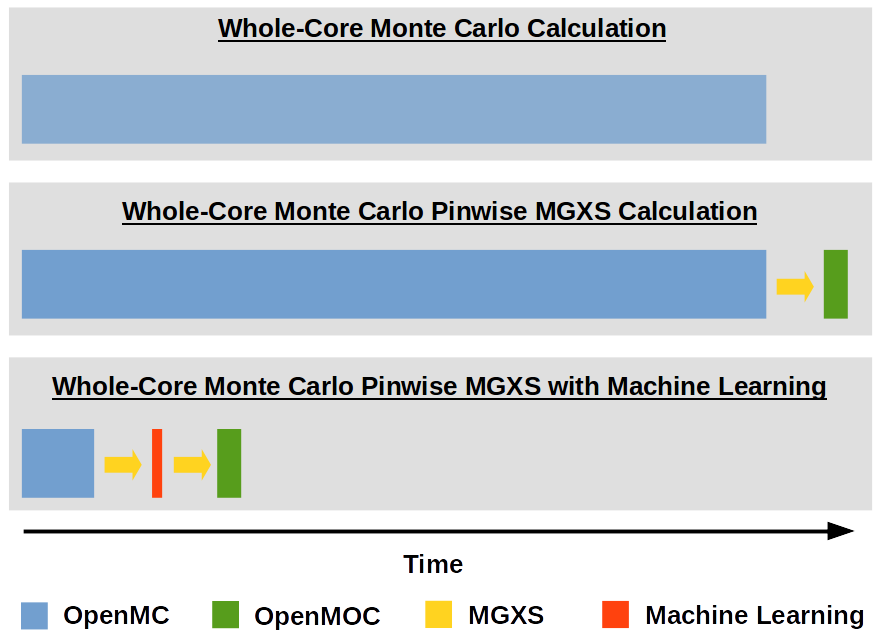
\includegraphics[width=0.6\linewidth]{figures/unsupervised/flow-chart}
\vspace{2mm}
\caption[Expected relative runtime for different homogenization schemes]{The expected relative runtime for the degenerate, \ac{LNS} and \textit{i}\ac{MGXS} spatial homogenization schemes with respect to a reference \ac{MC} calculation.}
\label{fig:chap10-flow-chart}
\end{figure}

This chapter begins by introducing a general latent variable model for \ac{MGXS} clustering which motivates \textit{i}\ac{MGXS} spatial homogenization in Sec.~\ref{sec:chap10-latent-model}. An overview of the \textit{i}\ac{MGXS} scheme is given in Sec.~\ref{sec:chap10-overview}, with in-depth presentations of the each stage of tally data pre-processing, including feature engineering (Sec.~\ref{sec:chap10-feature-engineer}), target selection (Sec.~\ref{sec:chap10-target-select}), feature transformation (Sec.~\ref{sec:chap10-feature-transform}), dimensionality reduction (Sec.~\ref{sec:chap10-dimensions-reduce}) and litmus tests (Sec.~\ref{sec:chap10-litmus}). Sec.~\ref{subsec:chap10-clustering} highlights a few statistical clustering algorithms which may be interchangeably employed within the code framework for i\ac{MGXS} implemented for this thesis. A few heuristics for unsupervised cluster model selection are discussed in Sec.~\ref{sec:chap10-model-select}. Sec.~\ref{sec:chap10-geometries} illustrates the material configurations produced by the \textit{i}\ac{MGXS} scheme for the heterogeneous \ac{PWR} benchmarks studied in this thesis. Finally, Sec.~\ref{sec:chap10-cluster} details two approaches used to evaluate the ideal and realized convergence rates of the \textit{i}\ac{MGXS} scheme. The eigenvalues and pin-wise fission and U-238 capture rates produced with the \textit{i}\ac{MGXS} scheme are evaluated in the following chapter.
  

%%%%%%%%%%%%%%%%%%%%%%%%%%%%%%%%%%%%%%%%%%%%%%%%%%%%%%%%%%%%%%%%%%%%%%%%%%%%%%%%
%\section{Latent Spectral Variable Model}
%\label{sec:chap10-lsvm}
%
%This section postulates the existence of a probability distribution from which pin-wise \ac{MGXS} are drawn when generated from Monte Carlo tallies. In particular, this section introduces a \textit{latent variable model} -- termed the \ac{LSVM} -- which encapsulates the spatial self-shielding effects in heterogeneous geometries that leads to clustering of pin-wise \ac{MGXS}. \ac{LSVM} inspires the development of the unsupervised statistical clustering methodology for spatial homogenization that is the topic of this and the following chapter. Latent variable models are a widely used theoretical construct for representing \textit{hidden variables} which parameterize the probability distributions that are thought to have produced some observed dataset. This section loosely follows Bishop's presentation of probabilistic mixture models~\cite{bishop2006pattern}, including the mathematical notation frequently employed by discussions of latent variable models in the statistics and machine learning literature. Sec.~\ref{subsec:chap10-lsvm-math} introduces the concept of latent spectral variables which dictate a parametrization of a mixture distribution which generated the pin-wise \ac{MGXS}. Sec.~\ref{subsec:chap10-lsvm-graph} illustrates \ac{LSVM} with a few graphical models.
%
%%Sec.~\ref{subsec:chap10-lsvm-additive-noise} begins by decompose \ac{MC} estimates for \ac{MGXS} into a multi-component additive noise model. 
%
%%%%%%%%%%%%%%%%%%%%%%%%%%%%%%%%%%%
%\subsection{Latent Spectral Variables}
%\label{subsec:chap10-lsvm-math}
%
%
%
%As shown in Chap.~\ref{chap:spatial}, spatial self-shielding effects from geometric heteoregneities leads to clustering of pin-wise \ac{MGXS}. This may 
%
%The \ac{MGXS} clustering effects induced by spatial self-shielding from various core heterogeneities, 
%
%\begin{align}
%\label{eqn:chap10-mgxs-offsets}
%\sigma_{k} &= \pi_{k,1}\Delta_{1} + \pi_{k,2}\Delta_{2} + \cdots + \pi_{k,M}\Delta_{M} \\
%&= \displaystyle\sum\limits_{m=1}^{M}\pi_{k,m}\Delta_{m}
%\end{align}
%
%
%
%As discussed in Sec.~\ref{sec:chap3-mgxs-gen}, the \ac{MGXS} tallied by \ac{MC} are random variables each with an estimated sample mean and variance. \ac{LSVM} describes the probability distribution that produced the population of \ac{MGXS} random variables for a particular type of material zone. In this thesis, \ac{LSVM} is used to describe the population of pin-wise microscopic \ac{MGXS} for all instances of fuel pins of a particular enrichment in a core geometry. For example, the tallied pin-wise microscopic \ac{MGXS} $\hat{\sigma}_{x,i,k,g}$ for some reaction $x$, nuclide $i$, fuel pin instance $k$ and energy group $g$ constitute the dataset produced by some probability distribution. \ac{LSVM} hypothesizes that the statistical process which generated the \ac{MGXS} dataset is a \textit{mixture model distribution} with $M$ mixture components. Each component $m$ is a normalized distribution $p(\hat{\sigma}_{x,i,k,g}; \boldsymbol{\theta}_{m})$ parameterized by vector $\boldsymbol{\theta}_{m}$, where for simplicity is assumed that all components are from the same parametric family of distributions\footnote{This restriction may not accurately characterize the mixtures components which generates pin-wise \ac{MGXS}, but is useful to simplify the number of symbols needed to introduces \ac{LSVM}.}\textsuperscript{,}\footnote{If the components are normal then $p(\hat{\sigma}_{x,i,k,g}; \boldsymbol{\theta}_{m}) = \mathcal{N}(\boldsymbol{\theta}_{m})$ with parameter vector $\boldsymbol{\theta}_{m} = \left[\mu_{m} \;\; \sigma_{m}\right]^{T}$.}. The components are combined in a linear superposition with \textit{mixing coefficients} $\pi_{m}$ to produce the mixture model distribution $f(\hat{\sigma}_{x,i,k,g})$:
%
%\begin{equation}
%\label{eqn:chap10-mix-model}
%f(\hat{\sigma}_{x,i,k,g}) = \displaystyle\sum\limits_{m=1}^{M} \pi_{m} p(\Delta_{m}; \boldsymbol{\theta}_{m})
%\end{equation}
%
%%\begin{equation}
%%\label{eqn:chap10-mix-model}
%%f(\hat{\sigma}_{x,i,k,g}) = \displaystyle\sum\limits_{m=1}^{M} \pi_{m} p(\hat{\sigma}_{x,i,k,g}; \boldsymbol{\theta}_{m})
%%\end{equation}
%
%\noindent where the coefficients ${\pi_{m}}$ are defined to sum to unity such that the model is normalized:
%
%%If each mixture has $N$ parameters (\textit{e.g}, $|\boldsymbol{\theta}| = N$), then $\boldsymbol{\Theta}$ is the $K \times N$ matrix of mixture model parameters, and $\boldsymbol{\Lambda}$ is the $K$-dimensional vector $\boldsymbol{\lambda} = \left[\lambda_{1} \;\; \lambda_{2} \;\; \dots \;\; \lambda_{m}\right]^{T}$ of mixing weights. The weights are defined to sum to unity such that the mixture model is normalized:
%
%\begin{equation}
%\label{eqn:chap10-mix-weights-norm}
%0 \le \pi_{m} \le 1 \;\;\; , \;\;\; \displaystyle\sum\limits_{m=1}^{M} \pi_{m} = 1
%\end{equation}
%
%The statistical model in Eqn.~\ref{eqn:chap10-mix-model} is a complete prescription for how the dataset of $\hat{\sigma}_{x,i,k,g}$ are generated for the population of fuel pins. In particular, \ac{LSVM} hypothesizes the existence of a \textit{latent spectral variable} $z_{k}$ for each fuel pin instance. Furthermore, \ac{LSVM} posits that the latent spectral variable may assume $Z$ integral values such that $z_{k} \in \{1, 2, \dots, Z\}$. From a practical standpoint, the latent spectral variable corresonds to the shape of the flux across energy group $g$ in fuel pin instance $k$\footnote{The shape of the flux across energy group $g$ cannot be directly observed from energy-integrated \ac{MC} tally data, and hence the spectral variable is a latent or hidden variable.}. \ac{LSVM} prescribes a one-to-one mapping from each possible value of the latent variable $z_{k}$ to a corresponding vector of mixing coefficients $\boldsymbol{\pi}(z_{k})$:
%
%\begin{equation}
%\label{eqn:chap10-mix-coeffs}
%\boldsymbol{\pi}(z_{k}) = \boldsymbol{\pi}_{k} = \left[\lambda_{1,k} \;\; \lambda_{2,k} \;\; \cdots \;\; \lambda_{m,k}\right]^{T}
%\end{equation}
%
%\noindent used to generate the dataset of $\hat{\sigma}_{x,i,k,g}$ according to the following stochastic process:
%
%\begin{equation}
%\label{eqn:chap10-lsvm}
%\hat{\sigma}_{x,i,k,g} \;\; \sim \;\; f(\hat{\sigma}_{x,i,k,g})
%\end{equation}
%
%%\ell \;\; &\sim \;\; \text{Multinomial}(p_{1}, p_{2}, \dots, p_{M}) \\
%% \boldsymbol{\lambda} \;\; &\sim \;\; \text{Categorical}(p_{1}, p_{2}, \dots, p_{M}) \\
%
%%\footnote{The symbol $\phi$ is adopted from the widely used notation for latent variables in the machine learning literature and should not be confused for the neutron flux.}
%
%
%%%%%%%%%%%%%%%%%%%%%%%%%%%%%%%%%%%%%%%%%%%%
%\subsection{An Additive Noise Model for MGXS}
%\label{subsec:chap10-lsvm-additive-noise}
%
%Additive noise models are useful theoretical construct widely considered in information theory to model many stochastic processes found in nature. This section introduces an additive noise model for \ac{MC} estimates for \ac{MGXS}. Consider an arbitrary propbability distribution $f_{x,i,k,g}(\cdot)$ from which the estimated pin-wise \ac{MGXS} $\hat{\sigma}_{x,i,k,g}$ (Eqn.~\ref{eqn:chap3-general-micro}) for reaction $x$, nuclide $i$, spatial zone $k$ and energy group $g$ are drawn:
%
%\begin{equation}
%\label{eqn:chap10-mgxs-draw}
%\hat{\sigma}_{x,i,k,g} \;\; \sim \;\; f_{x,i,k,g}(\hat{\sigma})
%\end{equation}
%
%\noindent The reaction $x$, nuclide $i$ and energy group $g$ subscripts may dropped for brevity:
%
%\begin{equation}
%\label{eqn:chap10-mgxs-draw-brevity}
%\hat{\sigma}_{k} \;\; \sim \;\; f_{k}(\hat{\sigma})
%\end{equation}
%
%An additive noise model may treat the \ac{MC} estimate for the \ac{MGXS} $\hat{\sigma}_{k}$ as the composition of the ``true'' \ac{MGXS} $\sigma_{k}$ (\textit{i.e.}, the expectation of $f(\hat{\sigma}_{k})$, or $\mathbb{E}[\hat{\sigma}_{k}]$) and a random ``noise'' term $\epsilon_{k}$. The noise $\epsilon_{k}$ is a random variable drawn from an arbitrary distribution $p(\epsilon; \boldsymbol{\theta}_{k})$ parameterized by $\boldsymbol{\theta}_{k}$ which represents the statistical uncertainty of the \ac{MC} estimate\footnote{If the \ac{MC} realizations are i.i.d. then the noise variables are normally distributed.}. The additive noise model for $\hat{\sigma}_{k}$ is then simply the sum of the true \ac{MGXS} and the random noise terms:
%
%\begin{align}
%\label{eqn:chap10-add-noise}
%\epsilon_{k} \;\; &\sim \;\; p(\epsilon; \boldsymbol{\theta}_{k}) \\
%\hat{\sigma}_{k} &= \sigma_{k} + \epsilon_{k}
%\end{align}
%
%As shown in Chap.~\ref{}, spatial self-shielding effects from geometric heteoregneities leads to clustering of pin-wise \ac{MGXS}. This may 
%
%The \ac{MGXS} clustering effects induced by spatial self-shielding from various core heterogeneities, 
%
%\begin{align}
%\label{eqn:chap10-mgxs-offsets}
%\sigma_{k} &= \pi_{k,1}\Delta_{1} + \pi_{k,2}\Delta_{2} + \cdots + \pi_{k,M}\Delta_{M} \\
%&= \displaystyle\sum\limits_{m=1}^{M}\pi_{k,m}\Delta_{m}
%\end{align}
%
%
%\begin{align}
%\label{eqn:chap10-mgxs-noise}
%\epsilon_{m} \;\; &\sim \;\; p(\epsilon; \boldsymbol{\theta}_{m}) \\
%\hat{\Delta}_{m} &= \Delta_{m} + \epsilon_{m}
%\end{align}
%
%compose the noise into different spectral effects
%
%\begin{align}
%\label{eqn:chap10-sum-noise}
%\hat{\sigma}_{k} &= \pi_{k,1}\hat{\Delta}_{1} + \pi_{k,2}\hat{\Delta}_{2} + \cdots + \pi_{k,M}\hat{\Delta}_{M} \\
%&= \pi_{k,1}\left(\Delta_{1} + \epsilon_{1}\right) + \pi_{k,2}\left(\Delta_{2} + \epsilon_{m}\right) + \cdots + \pi_{k,M}\left(\Delta_{M} + \epsilon_{m}\right) \\
%&= \displaystyle\sum\limits_{m=1}^{M}\pi_{k,m}\left(\Delta_{m} + \epsilon_{m}\right) \\
%&= \displaystyle\sum\limits_{m=1}^{M}\pi_{k,m}\Delta_{m} + \displaystyle\sum\limits_{m=1}^{M}\pi_{k,m}\epsilon_{m} \\
%% &= \sigma_{k} + \displaystyle\sum\limits_{m=1}^{M}\pi_{k,m}\epsilon_{m}
%\end{align}
%
%
%%%%%%%%%%%%%%%%%%%%%%%%%%%%%
%\subsection{Graphical Plate Notation}
%\label{subsec:chap10-lsvm-graph}
%
%\begin{figure}
%\centering
%\begin{tikzpicture}
%\tikzstyle{main}=[circle, minimum size = 8mm, thick, draw =black!80, node distance = 16mm]
%\tikzstyle{param}=[regular polygon, regular polygon sides=4, minimum size = 8mm, thick, draw =black!80, node distance = 16mm]
%  \node[param] (zk) [label=above:$z_k$] { };
%  \node[param] (theta) [left=of zk,label=left:$\boldsymbol{\Theta}$] { };
%  \node[main, fill = black!20] (sigma) [below=of zk, label=below:$\hat{\sigma}_{x,i,k,g}$] { };
%  \node[param] (pi) [left=of sigma,label=left:$\boldsymbol{\pi}$] { };
%   \draw[dagconn] (zk) to (sigma);
%   \draw[dagconn] (theta) to (sigma);
%   \draw[dagconn] (pi) to (sigma);
%   \node[plate=K, inner sep=20pt, fit=(zk) (sigma)] (plate1) {};
%\end{tikzpicture}
%\vspace{4mm}
%\caption[Graphical model for LSVM for a specific reactor configuration]{A graphical model to describe \ac{LSVM} for a specific reactor configuration.}
%\label{fig:chap10-lsvm-plate}
%\end{figure}
%
%\begin{figure}
%\centering
%\begin{tikzpicture}
%\tikzstyle{main}=[circle, minimum size = 8mm, thick, draw =black!80, node distance = 16mm]
%\tikzstyle{param}=[regular polygon, regular polygon sides=4, minimum size = 8mm, thick, draw =black!80, node distance = 16mm]
%  \node[param] (alpha) [label=above:$\boldsymbol{\alpha}$] { };
%  \node[main] (theta) [below left=of alpha,label=above:$\theta_{m}$] { };
%  \node[main] (pi) [below right=of alpha,label=above:$\pi_{m}$] { };
%  \node[param] (zk) [below=of theta,label=below:$z_k$] { };
%  \node[main, fill = black!20] (sigma) [below=of pi, label=below:$\hat{\sigma}_{x,i,k,g}$] { };
%   \draw[dagconn] (alpha) to (theta);
%   \draw[dagconn] (alpha) to (pi);
%   \draw[dagconn] (zk) to (sigma);
%   \draw[dagconn] (theta) to (sigma);
%   \draw[dagconn] (pi) to (sigma);
%   \node[plate=M, inner sep=20pt, fit=(theta) (pi)] (plate1) {};
%   \node[plate=K, inner sep=20pt, fit=(zk) (sigma)] (plate2) {};
%\end{tikzpicture}
%\vspace{4mm}
%\caption[Graphical model for LSVM for an arbitrary reactor configuration]{A graphical model to describe \ac{LSVM} for an arbitrary reactor configuration.}
%\label{fig:chap10-lsvm-plate-general}
%\end{figure}
%
%
%-we need to infer the latent variables $z_{k}$ for each fuel pin instance!!!
%-mention covariance between samples - the could be correlated
%-three goals:
%  -infer number of points/pins in each set
%  -infer conditional probabilities?
%  -assign each region to the most likely set?
%-is this section needed???
%-mention possibility of a multi-level latent variable model
%-mention bayesian approach to solving this using maximum likelihood


%%%%%%%%%%%%%%%%%%%%%%%%%%%%%%%%%%%%%%%%%%%%%%%%%%%%%%%%%%%%%%%%%%%%%%%%%%%%%%%
\section{Overview of \textit{i}MGXS}
\label{sec:chap10-overview}

The \textit{i}\ac{MGXS} spatial homogenization scheme is a multi-stage data processing \textit{pipeline}. The objective of the scheme is to infer the optimal assignment of cluster labels to fuel pin instances directly from \ac{MC} tally data. The cluster labels output by \textit{i}\ac{MGXS} are then used to generate track density-weighted \ac{MGXS} (see Sec.~\ref{subsec:chap9-lns-math}) for each cluster of fuel pin instances using the same process as that employed by \ac{LNS} homogenization (Eqn.~\ref{eqn:chap9-lns-micro}). The \textit{i}\ac{MGXS} methodology differs from the \ac{LNS} scheme in that it makes no consideration of the geometry and materials configuration and only examines tallied \ac{MC} tally data when assigning cluster labels to fuel pin instances.

A high-level overview of the various stages of the \textit{i}\ac{MGXS} data processing pipeline is illustrated in Fig.~\ref{fig:chap10-pipeline}. The \textit{i}\ac{MGXS} pipeline may be configured in various ways and this thesis makes no presumption that the incarnation presented in Fig.~\ref{fig:chap10-pipeline} is the best or most reliable version. Future work may develop schemes which improve upon the particular formulation of \textit{i}\ac{MGXS} presented in this thesis. Irregardless of the particular configuration, the overarching concept is that the \textit{i}\ac{MGXS} pipeline provides a \textit{mapping} between \ac{MC} tally data and cluster labels for each fuel pin\footnote{Similarly, the \ac{LNS} scheme defines a mapping between the combinatorial geometry and the cluster labels.}. Each of the six stages in Fig.~\ref{fig:chap10-pipeline} is detailed in the following sections of this thesis.

\begin{figure}[h!]
\centering
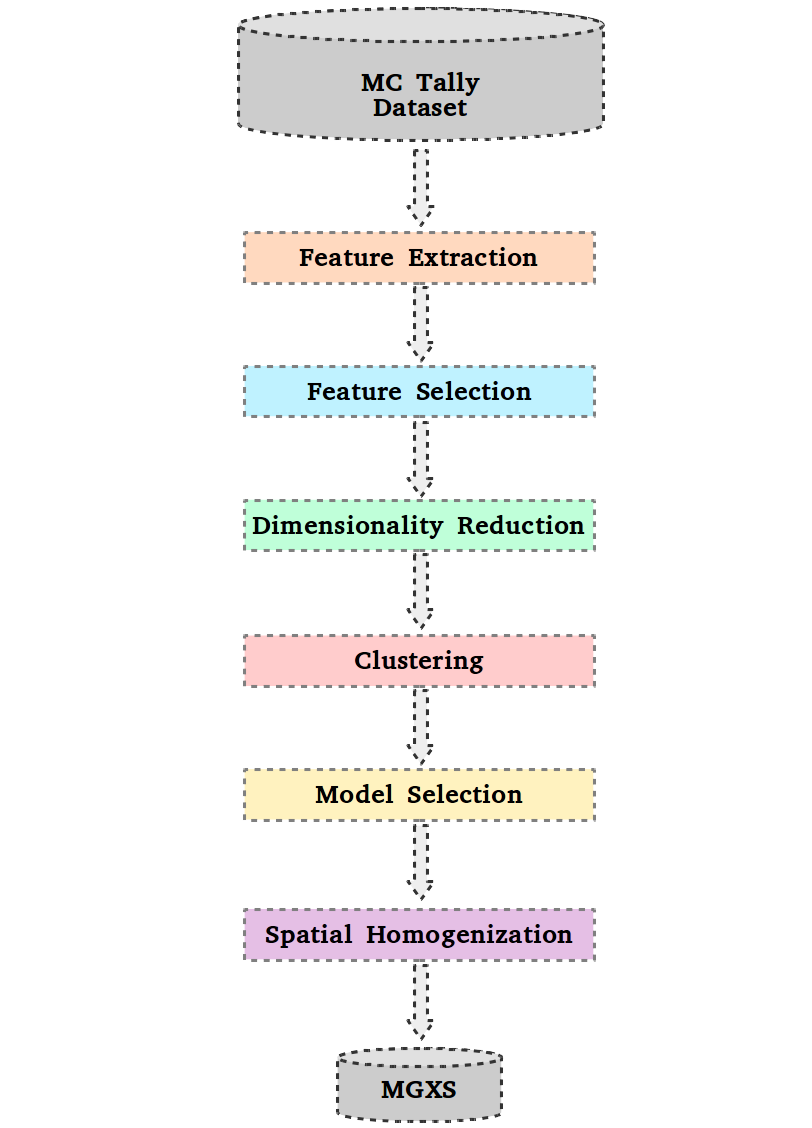
\includegraphics[width=0.655\linewidth]{figures/unsupervised/pipeline}
\vspace{2mm}
\caption[MGXS pipeline]{The multi-stage \textit{i}\ac{MGXS} data processing pipeline.}
\label{fig:chap10-pipeline}
\end{figure}


%%%%%%%%%%%%%%%%%%%%%%%%%%%%%%%%%%%%%%%%%%%%%%%%%%%%%%%%%%%%%%%%%%%%%%%%%%%%%%%
\section{Feature Extraction}
\label{sec:chap10-feature-extract}

The \textit{feature extraction} stage in the data processing pipeline in Fig.~\ref{fig:chap10-pipeline} builds \textit{features} from \ac{MC} tally data. In machine learning, features are simply variables which are used as inputs to a predictive model. Features may be engineered based upon prior domain knowledge or inferred from automated feature learning algorithms such as neural networks. In the context of \textit{i}\ac{MGXS}, features are restricted to tallies, or combinations of tallies, from \ac{MC} simulations which provide information about which fuel pin instances experience similar spatial self-shielding effects. For example, the pin-wise \ac{MGXS} $\hat{\sigma}_{x,i,k,g}$ themselves may be used as features since they exhibit the very clustering effect which \textit{i}\ac{MGXS} attempts to predict\footnote{Using the pin-wise \ac{MGXS} as the only feature(s) for unsupervised clustering would be equivalent to specifying boundaries between the samples illustrated in the rug plots in Sec.~\ref{subsec:chap9-histograms}.}. Other tallied quantities may also be used as features for predicting which fuel pin instances have similarly self-shielded \ac{MGXS}. The goal of extracting \textit{i}\ac{MGXS} features is to enable machine learning algorithms to identify \ac{MGXS} clusters as quickly as possible from ``noisy'' or unconverged tally data.

The \textit{i}\ac{MGXS} scheme splits the \ac{MC} tally dataset up into \textit{samples} for each particular instance $k$ of a fuel pin as illustrated in Fig.~\ref{fig:chap10-feature-extract}. A \textit{sample} is a random vector with $J$ entries for each feature $\hat{f}_{j,k}$ corresponding to a particular instance $k$ of a fuel pin. A sample may be comprised of features derived from \ac{MC} tally data for one or multiple nuclides, energy groups and/or reaction types. Ideally, the features should maximize the \textit{separation distance} in feature space $\{f_{1}, f_{2}, \dots, f_{J}\}$ between samples from the same cluster. Since features in \textit{i}\ac{MGXS} are tallied quantities from \ac{MC} simulations, some samples may include ``outlier'' feature realizations which take on values far removed from the ``true'' value of the feature\footnote{The ``true'' values are the expected values for each feature.}. Outliers may result in the incorrect assignment of cluster labels to fuel pin instances. The predictive models used in \textit{i}\ac{MGXS} are trained with the complete vector of features in order to mitigate the sensitivity of the models to outlier features and minimize the frequency of mis-labeled cluster assignments.

\begin{figure}[h!]
\centering
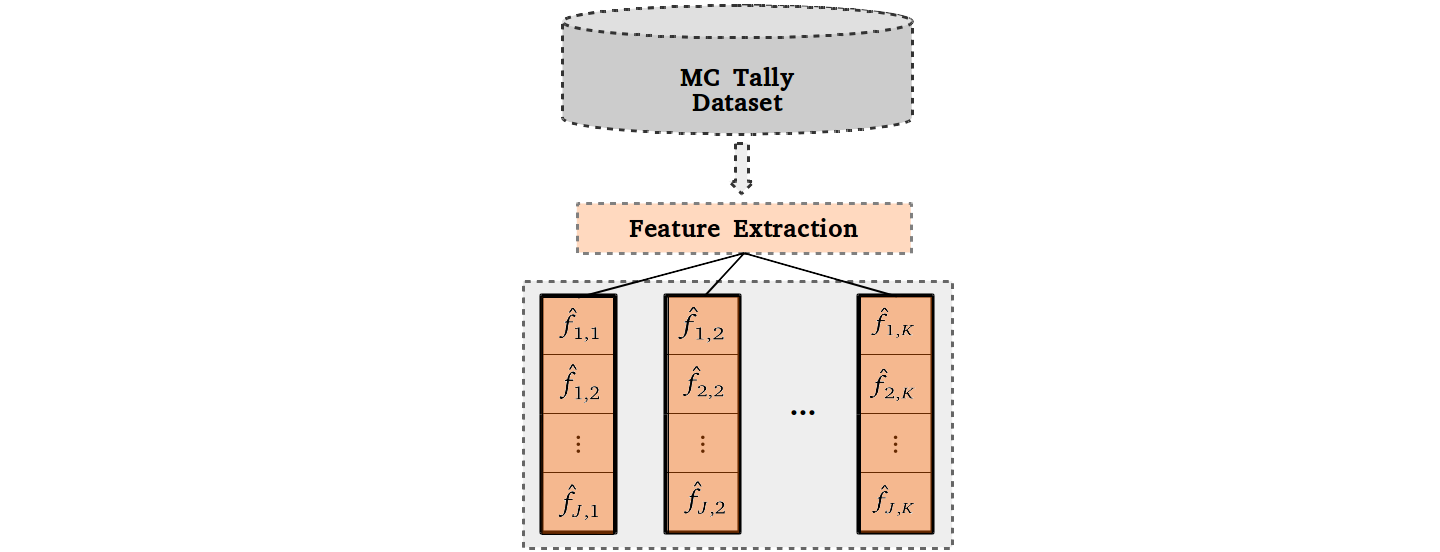
\includegraphics[width=0.9\linewidth]{figures/unsupervised/features/engineering/extract}
\vspace{2mm}
\caption[\textit{i}MGXS sample feature extraction]{\textit{i}\ac{MGXS} extracts feature vectors for each sample (fuel pin instance).}
\label{fig:chap10-feature-extract}
\end{figure}

In addition, it should be noted that features may not necessarily be defined for the same energy group structure as the \ac{MGXS} one wishes to cluster. For example, some or all features may be tallied on a relatively coarse energy group structure in order to minimize their \ac{MC} statistical uncertainties. It is in fact be beneficial to tally features in few groups in order to identify clusters with fewer \ac{MC} particle histories than would needed to distinguish structure from ``noisy'' fine group features.
These coarse group features may be input to a clustering algorithm for spatial homogenization of pin-wise \ac{MGXS} defined on a fine(r) energy group structure. For example, the following sections and chapters cluster features defined for a coarse 2-group structure in order to assign each fuel pin to a cluster for spatial homogenization of the ``fine'' 70-group pin-wise \ac{MGXS} data needed to minimize reaction rate errors to 1 -- 2\% or less.

The following sections introduce the features employed by \textit{i}\ac{MGXS} in this and the following chapter. These include the pin-wise \ac{MGXS} and their statistical uncertainties (Sec.~\ref{subsec:chap10-stat-uncertainty}), as well as features referred to as fractional reactivites (Sec.~\ref{subsec:chap10-frac-reactivity}), spectral indices (Sec.~\ref{subsec:chap10-spec-index}), nuclide fractions (Sec.~\ref{subsec:chap10-nuclide-frac}) and total fractions (Sec.~\ref{subsec:chap10-tot-frac}). Each feature is specific to a fuel pin instance, and may further be distinguished for one or more nuclides, energy groups and/or reaction types. Each feature is presented with accompanying illustrations generated using a custom-built tool to visualize \textit{i}\ac{MGXS} features~\cite{abel2016bokeh}, and which correspond to the 1.6\% enriched fuel assembly benchmark.

%The clustering algoritms used in \textit{i}\ac{MGXS} may more easily identify clusters from the less ``noisy'' feature data, and the cluster labels used to spatially homogenize fine(r) group pin-wise \ac{MGXS}. 

%first paragraph: motivationa 
%  -could cluster multiple microscopic \ac{MGXS} simultaneously - nuclides, reactions, groups

%%%%%%%%%%%%%%%%%%%%%%%%%%%%%%%%%%%%%%%%%
\subsection{MGXS Statistical Uncertainty}
\label{subsec:chap10-stat-uncertainty}

The statistical uncertainty for each pin-wise \ac{MGXS} may be a useful feature to indicate clustering effects. In particular, the standard deviation of the sample mean is easily obtained from OpenMC tallies and can be incldued in the feature vector for each fuel pin instance. The intuition behind this is that the track densities -- and therefore, the statistical uncertainties -- in different fuel pins may reflect the spatial self-shielding effects experienced by different types of fuel pins. For example, the thermal flux track density will vary for fuel pins with differential moderation from \acp{CRGT}, reflectors, etc., which may present itself through a systematic clustering of the statistical uncertainties. Similarly, the track density will vary for fuel pins which experience varying degrees of spatial self-shielding in U-238 resonance groups -- which greatly impacts the resultant \ac{MGXS} in those groups -- and may be identifiable in the \ac{MGXS} uncertainties.

The statistical uncertainty feature is illustrated with scatter plots in Figs.~\ref{fig:chap10-fiss-mean-std} and~\ref{fig:chap10-capt-mean-std} for 2-group U-235 fission and U-238 capture \ac{MGXS} data, respectively. The scatter plots include a single data point for each of the 264 fuel pins in the 1.6\% enriched fuel assembly benchmark. The $x$ and $y$ coordinates correspond to the tallied \ac{MGXS} means $\hat{\sigma}_{x,i,k,g}$ and standard deviations $\sigma_{\hat{\sigma}_{x,i,k,g}}$ in units of barns, respectively. The complete datasets are illustrated in Figs.~\ref{fig:chap10-fiss-mean-std-mgxs} and~\ref{fig:chap10-capt-mean-std-mgxs}. The interactive \textit{i}\ac{MGXS} visualization tool was used to select clusters of \ac{MGXS} and plot the geometry to indicate the associated fuel pins, as displayed in Figs.~\Crefrange{fig:chap10-fiss-mean-std-geom-2}{fig:chap10-fiss-mean-std-mgxs-3} and~\Crefrange{fig:chap10-capt-mean-std-geom-2}{fig:chap10-capt-mean-std-mgxs-3} for the fission and capture \ac{MGXS}, respectively. The figures illustrate that the U-235 \ac{MGXS} uncertainties are smallest for the fuel pins with the most differential moderation (\textit{i.e.}, pin facially adjacent to \acp{CRGT}) and a relatively larger thermal flux track density. In contrast, the U-238 capture \ac{MGXS} uncertainties are largest for those pins with the most differential moderation due to the smaller fast-to-thermal flux ratio in these pins.

Notwithstanding the motivation to use the statistical uncertainties, there are also potential challenges associated with this approach. First, it would be possible for two different fuel pin instances to experience the same flux shape -- and therefore have the same \ac{MGXS} -- but very different flux magnitudes. Although the \ac{MGXS} uncertainties for the two pins would be very different, this would not accurately reflect the fact that the two pins should ideally be assigned to the same \ac{MGXS} cluster. Furthermore, error propagation theory only approximates the \ac{MGXS} uncertainties since it neglects the covariance between reaction rate and flux tallies. This approximation overestimates the \ac{MGXS} uncertainties since the reaction rate and flux tallies are highly correlated. As a result, the uncertainties may not exhibit systematic trends with poorly converged \ac{MC} data since the uncertainties will be larger than their ``true'' values. However, these are not reasons to eliminate the uncertainties as a possible feature; rather, it incites the need for robust feature selection as discussed in Sec.~\ref{sec:chap10-feature-select}.

%\begin{equation}
%\label{eqn:chap10-rel-err}
%\eta_{x,i,k,g} = \frac{\sigma_{\hat{\sigma}_{x,i,k,g}}}{\hat{\sigma}_{x,i,k,g}}
%\end{equation}

\begin{figure}[h!]
\centering
\begin{subfigure}{0.45\textwidth}
  \centering
  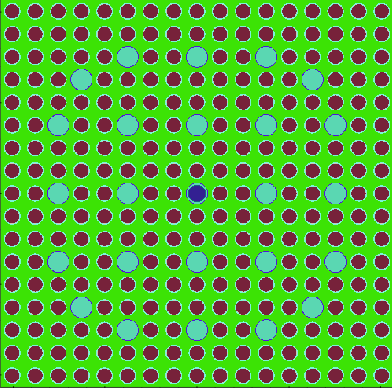
\includegraphics[width=0.9\linewidth]{figures/unsupervised/features/assm-16/geometry}
  \caption{}
  \label{fig:chap10-fiss-mean-std-geom}
\end{subfigure}%
\begin{subfigure}{0.45\textwidth}
  \centering
  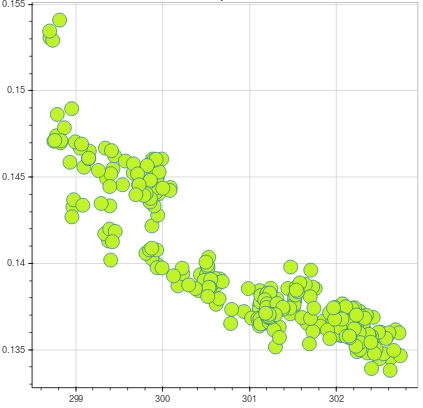
\includegraphics[width=0.9\linewidth]{figures/unsupervised/features/assm-16/u235-fiss/mean-std/mgxs}
  \caption{}
  \label{fig:chap10-fiss-mean-std-mgxs}
\end{subfigure}
\begin{subfigure}{0.45\textwidth}
  \centering
  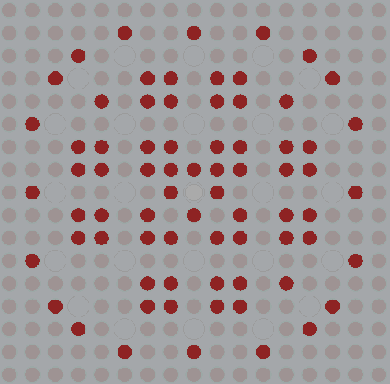
\includegraphics[width=0.9\linewidth]{figures/unsupervised/features/assm-16/u235-fiss/mean-std/geometry-2}
  \caption{}
  \label{fig:chap10-fiss-mean-std-geom-2}
\end{subfigure}%
\begin{subfigure}{0.45\textwidth}
  \centering
  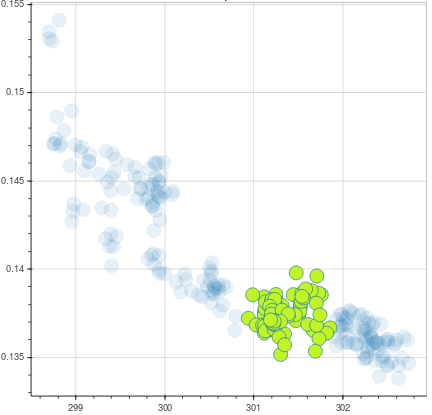
\includegraphics[width=0.9\linewidth]{figures/unsupervised/features/assm-16/u235-fiss/mean-std/mgxs-2}
  \caption{}
  \label{fig:chap10-fiss-mean-std-mgxs-2}
\end{subfigure}
\begin{subfigure}{0.45\textwidth}
  \centering
  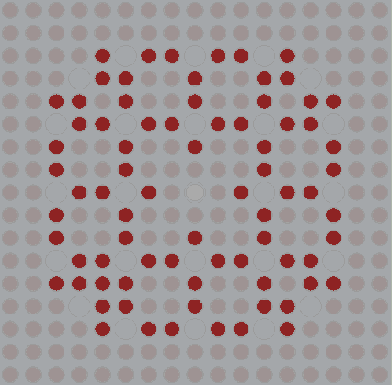
\includegraphics[width=0.9\linewidth]{figures/unsupervised/features/assm-16/u235-fiss/mean-std/geometry-3}
  \caption{}
  \label{fig:chap10-fiss-mean-std-geom-3}
\end{subfigure}%
\begin{subfigure}{0.45\textwidth}
  \centering
  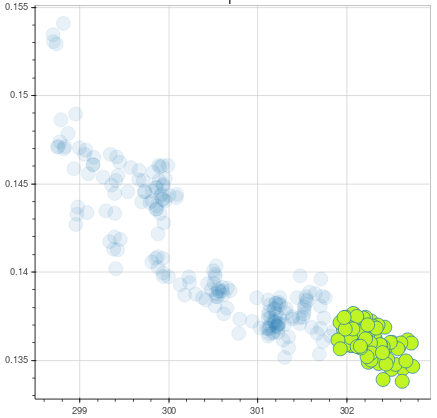
\includegraphics[width=0.9\linewidth]{figures/unsupervised/features/assm-16/u235-fiss/mean-std/mgxs-3}
  \caption{}
  \label{fig:chap10-fiss-mean-std-mgxs-3}
\end{subfigure}
\caption[Clustering of U-235 fission MGXS standard deviations]{Scatter plots of the pin-wise U-235 fission (group 2 of 2) \ac{MGXS} means ($x$) and standard deviations ($y$) for the 1.6\% enriched fuel assembly.}
\label{fig:chap10-fiss-mean-std}
\end{figure}

\clearpage

\begin{figure}[h!]
\centering
\begin{subfigure}{0.45\textwidth}
  \centering
  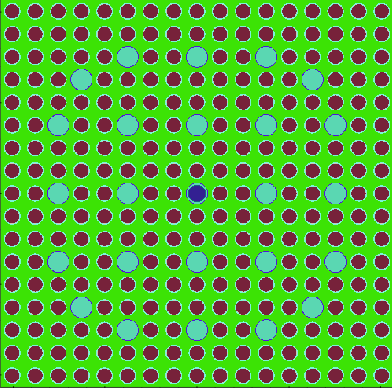
\includegraphics[width=0.9\linewidth]{figures/unsupervised/features/assm-16/geometry}
  \caption{}
  \label{fig:chap10-capt-mean-std-geom}
\end{subfigure}%
\begin{subfigure}{0.45\textwidth}
  \centering
  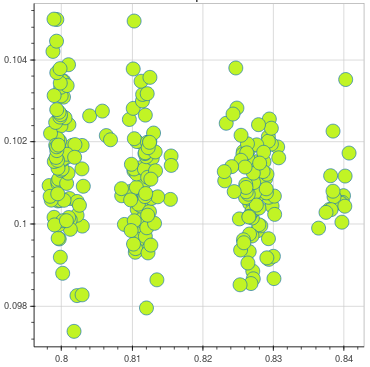
\includegraphics[width=0.9\linewidth]{figures/unsupervised/features/assm-16/u238-capt/mean-std/mgxs}
  \caption{}
  \label{fig:chap10-capt-mean-std-mgxs}
\end{subfigure}
\begin{subfigure}{0.45\textwidth}
  \centering
  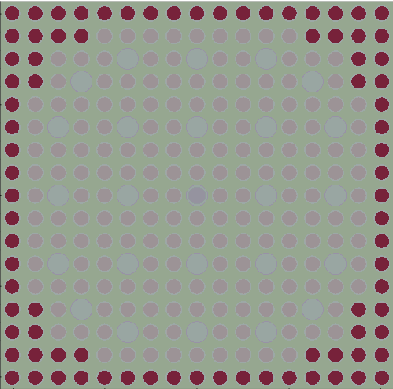
\includegraphics[width=0.9\linewidth]{figures/unsupervised/features/assm-16/u238-capt/mean-std/geometry-2}
  \caption{}
  \label{fig:chap10-capt-mean-std-geom-2}
\end{subfigure}%
\begin{subfigure}{0.45\textwidth}
  \centering
  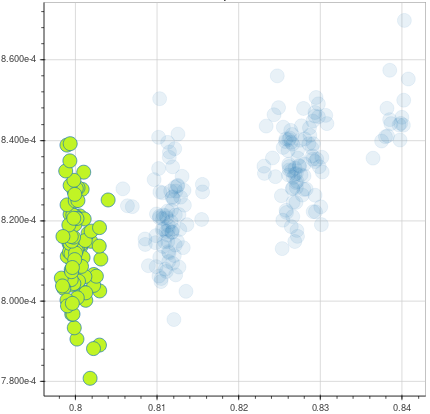
\includegraphics[width=0.9\linewidth]{figures/unsupervised/features/assm-16/u238-capt/mean-std/mgxs-2}
  \caption{}
  \label{fig:chap10-capt-mean-std-mgxs-2}
\end{subfigure}
\begin{subfigure}{0.45\textwidth}
  \centering
  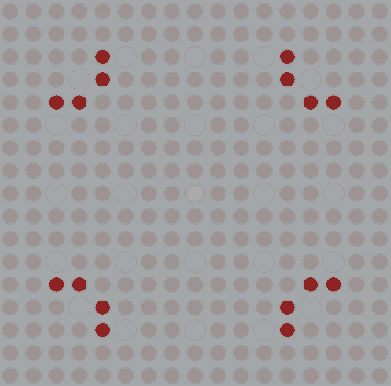
\includegraphics[width=0.9\linewidth]{figures/unsupervised/features/assm-16/u238-capt/mean-std/geometry-3}
  \caption{}
  \label{fig:chap10-capt-mean-std-geom-3}
\end{subfigure}%
\begin{subfigure}{0.45\textwidth}
  \centering
  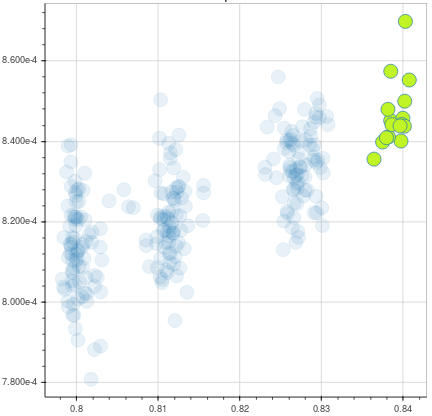
\includegraphics[width=0.9\linewidth]{figures/unsupervised/features/assm-16/u238-capt/mean-std/mgxs-3}
  \caption{}
  \label{fig:chap10-capt-mean-std-mgxs-3}
\end{subfigure}
\caption[Clustering of U-238 capture MGXS standard deviations]{Scatter plots of the pin-wise U-238 capture (group 1 of 2) \ac{MGXS} means ($x$) and standard deviations ($y$) for the 1.6\% enriched fuel assembly.}
\label{fig:chap10-capt-mean-std}
\end{figure}

\clearpage

%%%%%%%%%%%%%%%%%%%%%%%%%%%%%%%%%%
\subsection{Fractional Reactivity}
\label{subsec:chap10-frac-reactivity}

The \textit{fractional reactivity} compares the fission reaction rates for the population of fuel pins in a core geometry. This feature hypothesizes that fuel pins with similar spatial self-shielding effects have similar fission rates. This may be a valid assumption for simple geometries such as fuel assemblies and colorsets with all reflective/periodic \acp{BC}, but may not be true for benchmarks such as \ac{BEAVRS} with large globally-varying power tilts due to leakage. The fission rate statistical uncertainties will necessarily be smaller than those for the microscopic \ac{MGXS} since they are energy-integrated and summed across nuclides. As a result, clustering may emerge from ``noisy'' \ac{MC} fission rate tallies more quickly than is possible for tallies for single energy groups and/or nuclides.

Although the pin-wise fission rates may used directly as a feature, the \textit{i}\ac{MGXS} implementation in this thesis normalizes the pin-wise fission rates to the globally-integrated absorption rate in the fuel as follows:

\begin{equation}
\label{eqn:chap10-frac-reactivity}
\hat{\alpha}_{k} = \frac{\displaystyle\sum\limits_{g=1}^{G}\nu\hat{\Sigma}_{f,i,k,g}\hat{\phi}_{k,g}}{\displaystyle\sum\limits_{k=1}^{K}\displaystyle\sum\limits_{g=1}^{G}\hat{\Sigma}_{a,i,k,g}\hat{\phi}_{k,g}} \times 10^{5}
\end{equation}

\noindent The normalized fractional reactivity $\hat{\alpha}_{k}$  is multiplied by 10$^{5}$ so that it may be reported in the familiar reactivity units of per cent mille (pcm)\footnote{It might be preferable to equivalently normalize the fission rates to the mean. The normalization factor is a matter of analyst preference and does not impact the predictions made by statistical clustering algorithms if the features are standardized as discussed in Sec.~\ref{sec:chap10-feature-transform}.}. It is important to note that the denominator in Eqn.~\ref{eqn:chap10-frac-reactivity} encompasses all fuel pins of all compositions (\textit{e.g.}, enrichments) in the core geometry, but does not include absorption in the moderator, clad, \acp{BP}, etc. As a result, the fractional reactivity as defined by this thesis is not indicative of the global reactivity, but rather the reactivity restricted to the fuel.

The fractional reactivity feature is illustrated with scatter plots in Figs.~\ref{fig:chap10-fiss-mean-pcm} and~\ref{fig:chap10-capt-mean-pcm} for 2-group U-235 fission and U-238 capture \ac{MGXS} data, respectively. The scatter plots include a single data point for each of the 264 fuel pins in the 1.6\% enriched fuel assembly benchmark. The $x$ and $y$ coordinates correspond to the tallied \ac{MGXS} means $\hat{\sigma}_{x,i,k,g}$ and normalized fractional reactivities $\hat{\alpha}_{k}$ in units of barns and \ac{pcm}, respectively. The complete datasets are illustrated in Figs.~\ref{fig:chap10-fiss-mean-pcm-mgxs} and~\ref{fig:chap10-capt-mean-pcm-mgxs}. The interactive \textit{i}\ac{MGXS} visualization tool was used to select clusters of \ac{MGXS} and plot the geometry to indicate the associated fuel pins, as displayed in Figs.~\Crefrange{fig:chap10-fiss-mean-pcm-geom-2}{fig:chap10-fiss-mean-pcm-mgxs-3} and~\Crefrange{fig:chap10-capt-mean-pcm-geom-2}{fig:chap10-capt-mean-pcm-mgxs-3} for the fission and capture \ac{MGXS}, respectively. 

The scatter plots illustrate the highly linear relationship between the U-235 fission \ac{MGXS} and fractional reactivities; those pins facially and corner adjacent to distinct \acp{CRGT} have both the largest fission \ac{MGXS} and fission rates due to the differential moderation of the neighboring \acp{CRGT} (at least for this benchmark). The clustering of U-238 capture \ac{MGXS} generally indicates a similar proportional relationship with fractional reactivity. Perhaps more importantly, Fig.~\ref{fig:chap10-mean-pcm} also makes it possible to distinguish ``sub-clusters'' within each of the four primary clusters of U-238 capture \ac{MGXS}. Although the sub-clusters within a primary cluster have similar \ac{MGXS}\footnote{The track density-weighted average \ac{MGXS} for the sub-clusters would be relatively similar.}, there is some variation due to subtle differences in the spatial self-shielding experienced by the pins in the primary cluster.

The visualizations highlight the \textit{hierarchical} nature of spatial self-shielding effects: some factors are most important and induce primary clusters (\textit{i.e.}, whether a fuel pin is adjacent to zero, one or two \acp{CRGT}), while other factors are less consequential yet still induce sub-clusters (\textit{i.e.}, the type adjacency of neighboring \acp{CRGT}). The hierarchy of spatial self-shielding effects will grow increasingly intricate with the size and complexity of the reactor configuration, further motivating the importance for an unsupervised methodology like \textit{i}\ac{MGXS} to identify \ac{MGXS} clustering for arbitrary core geometries.

\begin{figure}[h!]
\centering
\begin{subfigure}{0.45\textwidth}
  \centering
  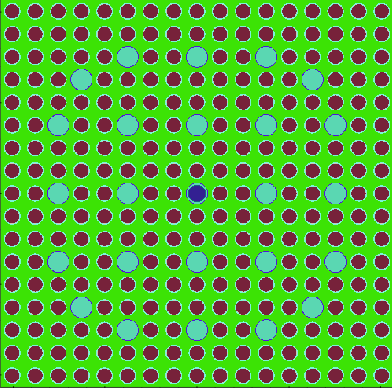
\includegraphics[width=0.9\linewidth]{figures/unsupervised/features/assm-16/geometry}
  \caption{}
  \label{fig:chap10-fiss-mean-pcm-geom}
\end{subfigure}%
\begin{subfigure}{0.45\textwidth}
  \centering
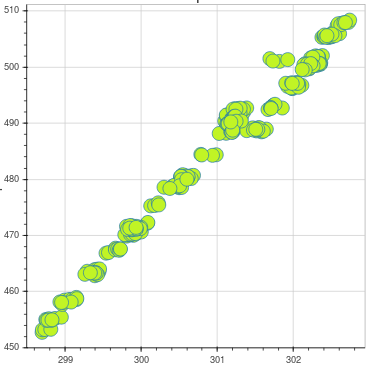
\includegraphics[width=0.9\linewidth]{figures/unsupervised/features/assm-16/u235-fiss/mean-pcm/mgxs}
  \caption{}
  \label{fig:chap10-fiss-mean-pcm-mgxs}
\end{subfigure}
\begin{subfigure}{0.45\textwidth}
  \centering
  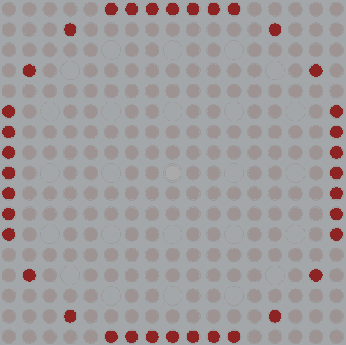
\includegraphics[width=0.9\linewidth]{figures/unsupervised/features/assm-16/u235-fiss/mean-pcm/geometry-2}
  \caption{}
  \label{fig:chap10-fiss-mean-pcm-geom-2}
\end{subfigure}%
\begin{subfigure}{0.45\textwidth}
  \centering
  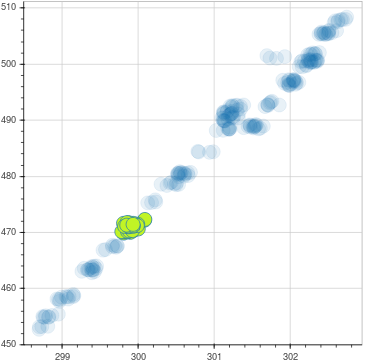
\includegraphics[width=0.9\linewidth]{figures/unsupervised/features/assm-16/u235-fiss/mean-pcm/mgxs-2}
  \caption{}
  \label{fig:chap10-fiss-mean-pcm-mgxs-2}
\end{subfigure}
\begin{subfigure}{0.45\textwidth}
  \centering
  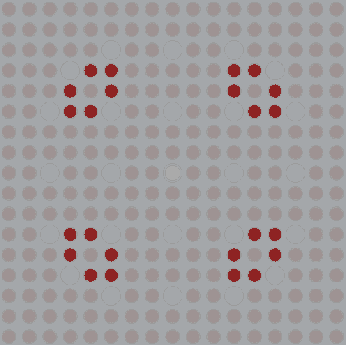
\includegraphics[width=0.9\linewidth]{figures/unsupervised/features/assm-16/u235-fiss/mean-pcm/geometry-3}
  \caption{}
  \label{fig:chap10-fiss-mean-pcm-geom-3}
\end{subfigure}%
\begin{subfigure}{0.45\textwidth}
  \centering
  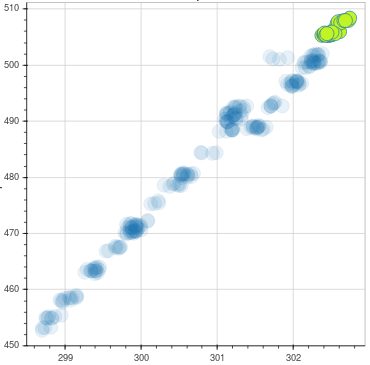
\includegraphics[width=0.9\linewidth]{figures/unsupervised/features/assm-16/u235-fiss/mean-pcm/mgxs-3}
  \caption{}
  \label{fig:chap10-fiss-mean-pcm-mgxs-3}
\end{subfigure}
\caption[Clustering of U-235 fission MGXS fractional reactivities]{Scatter plots of the pin-wise U-235 fission (group 2 of 2) \ac{MGXS} means ($x$) and fractional reactivities ($y$) for the 1.6\% enriched fuel assembly.}
\label{fig:chap10-fiss-mean-pcm}
\end{figure}

\clearpage

\begin{figure}[h!]
\centering
\begin{subfigure}{0.45\textwidth}
  \centering
  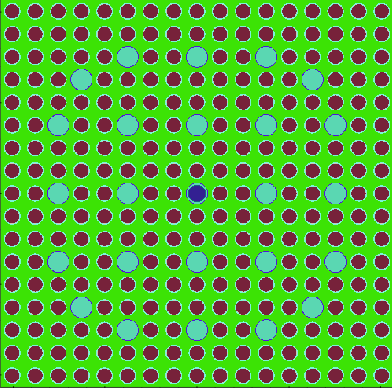
\includegraphics[width=0.9\linewidth]{figures/unsupervised/features/assm-16/geometry}
  \caption{}
  \label{fig:chap10-capt-mean-pcm-geom}
\end{subfigure}%
\begin{subfigure}{0.45\textwidth}
  \centering
  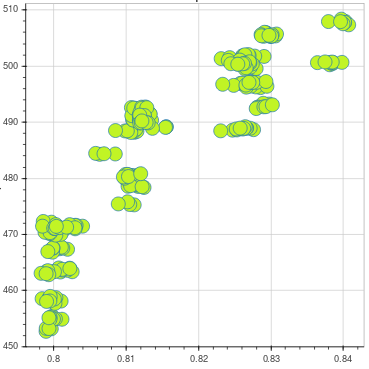
\includegraphics[width=0.9\linewidth]{figures/unsupervised/features/assm-16/u238-capt/mean-pcm/mgxs}
  \caption{}
  \label{fig:chap10-capt-mean-pcm-mgxs}
\end{subfigure}
\begin{subfigure}{0.45\textwidth}
  \centering
  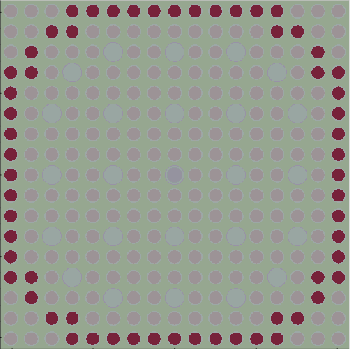
\includegraphics[width=0.9\linewidth]{figures/unsupervised/features/assm-16/u238-capt/mean-pcm/geometry-2}
  \caption{}
  \label{fig:chap10-capt-mean-pcm-geom-2}
\end{subfigure}%
\begin{subfigure}{0.45\textwidth}
  \centering
  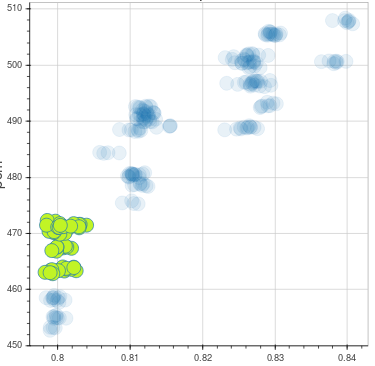
\includegraphics[width=0.9\linewidth]{figures/unsupervised/features/assm-16/u238-capt/mean-pcm/mgxs-2}
  \caption{}
  \label{fig:chap10-capt-mean-pcm-mgxs-2}
\end{subfigure}
\begin{subfigure}{0.45\textwidth}
  \centering
  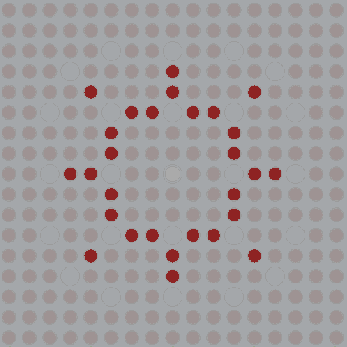
\includegraphics[width=0.9\linewidth]{figures/unsupervised/features/assm-16/u238-capt/mean-pcm/geometry-3}
  \caption{}
  \label{fig:chap10-capt-mean-pcm-geom-3}
\end{subfigure}%
\begin{subfigure}{0.45\textwidth}
  \centering
  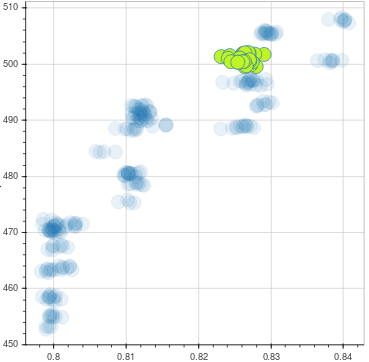
\includegraphics[width=0.9\linewidth]{figures/unsupervised/features/assm-16/u238-capt/mean-pcm/mgxs-3}
  \caption{}
  \label{fig:chap10-capt-mean-pcm-mgxs-3}
\end{subfigure}
\caption[Clustering of U-238 capture MGXS fractional reactivities]{Scatter plots of the pin-wise U-238 capture (group 1 of 2) \ac{MGXS} means ($x$) and fractional reactivities ($y$) for the 1.6\% enriched fuel assembly.}
\label{fig:chap10-capt-mean-pcm}
\end{figure}

\clearpage

%%%%%%%%%%%%%%%%%%%%%%%%%%%	
\subsection{Spectral Index}
\label{subsec:chap10-spec-index}

The \textit{spectral index} compares the ratio of energy-integrated U-238 capture to U-235 fission reaction rates in each fuel pin. The \textit{i}\ac{MGXS} implementation in this thesis computes spectral indices as follows:

\begin{equation}
\label{eqn:chap10-spec-index-u238-capt}
\hat{\beta}_{k} = \frac{\displaystyle\sum\limits_{g=1}^{G}\hat{\sigma}_{\gamma,k,g}^{238}\hat{\phi}_{k,g}}{\displaystyle\sum\limits_{g=1}^{G}\hat{\sigma}_{f,k,g}^{235}\hat{\phi}_{k,g}}
\end{equation}

\noindent where $\hat{\sigma}_{\gamma,k,g}^{238}$ and $\hat{\sigma}_{f,k,g}^{235}$ are the microscopic U-238 radiative capture and U-235 fission production \ac{MGXS} for fuel pin instance $k$ and energy group $g$, respectively\footnote{The U-235 fission and fission production \ac{MGXS} may be used interchangeably in Eqn.~\ref{eqn:chap10-spec-index-u238-capt} with no impact on the predictions made by unsupervised statistical clustering algorithms.}. This feature postulates that the capture-to-fission ratio will significantly vary for fuel pins and energy groups with different spatial self-shielding effects. The spectral index is especially relevant since it accounts for relative differences in the U-238 capture rates, which previous chapters showed can only be accurately computed if an appropriate pin-wise spatial homogenization scheme is used. Unlike the fractional reactivity, the spectral index may identify pins with similar flux shapes but very different flux magnitudes since it is the ratio of two pin-wise reaction rates.

The spectral index feature is illustrated with scatter plots in Figs.~\ref{fig:chap10-fiss-mean-spect-ind} and~\ref{fig:chap10-capt-mean-spect-ind} for 2-group U-235 fission and U-238 capture \ac{MGXS} data, respectively. The scatter plots include a single data point for each of the 264 fuel pins in the 1.6\% enriched fuel assembly benchmark. The $x$ and $y$ coordinates correspond to the tallied \ac{MGXS} means $\hat{\sigma}_{x,i,k,g}$ and spectral indices $\hat{\beta}_{k}$, respectively. The complete datasets are illustrated in Figs.~\ref{fig:chap10-fiss-mean-spect-ind-mgxs} and~\ref{fig:chap10-capt-mean-spect-ind-mgxs}. The interactive \textit{i}\ac{MGXS} visualization tool was used to select clusters of \ac{MGXS} and plot the geometry to indicate the associated fuel pins, as displayed in Figs.~\Crefrange{fig:chap10-fiss-mean-spect-ind-geom-2}{fig:chap10-fiss-mean-spect-ind-mgxs-3} and~\Crefrange{fig:chap10-capt-mean-spect-ind-geom-2}{fig:chap10-capt-mean-spect-ind-mgxs-3} for the fission and capture \ac{MGXS}, respectively. 

\begin{figure}[h!]
\centering
\begin{subfigure}{0.42\textwidth}
  \centering
  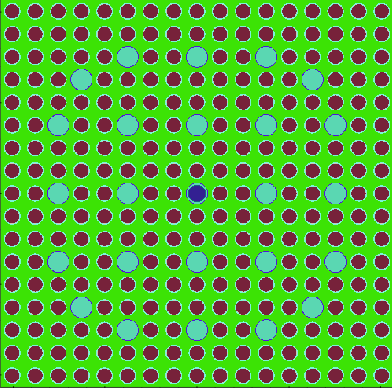
\includegraphics[width=0.8\linewidth]{figures/unsupervised/features/assm-16/geometry}
  \caption{}
  \label{fig:chap10-fiss-mean-spect-ind-geom}
\end{subfigure}%
\begin{subfigure}{0.45\textwidth}
  \centering
  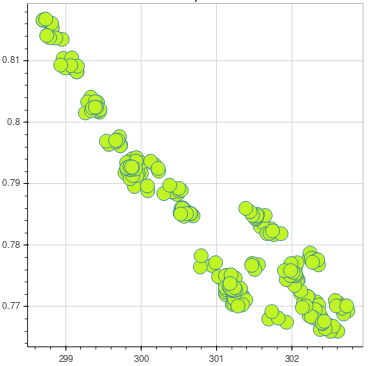
\includegraphics[width=0.9\linewidth]{figures/unsupervised/features/assm-16/u235-fiss/mean-spect-ind-sum/mgxs}
  \caption{}
  \label{fig:chap10-fiss-mean-spect-ind-mgxs}
\end{subfigure}
\begin{subfigure}{0.45\textwidth}
  \centering
  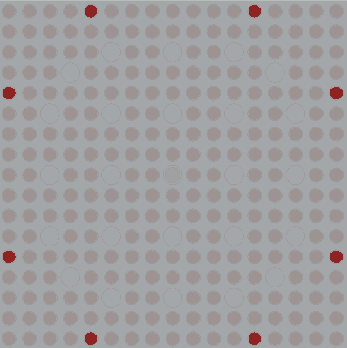
\includegraphics[width=0.9\linewidth]{figures/unsupervised/features/assm-16/u235-fiss/mean-spect-ind-sum/geometry-2}
  \caption{}
  \label{fig:chap10-fiss-mean-spect-ind-geom-2}
\end{subfigure}%
\begin{subfigure}{0.45\textwidth}
  \centering
  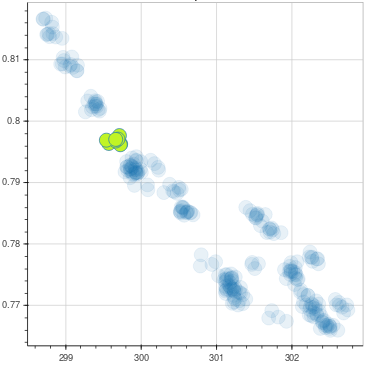
\includegraphics[width=0.9\linewidth]{figures/unsupervised/features/assm-16/u235-fiss/mean-spect-ind-sum/mgxs-2}
  \caption{}
  \label{fig:chap10-fiss-mean-spect-ind-mgxs-2}
\end{subfigure}
\begin{subfigure}{0.45\textwidth}
  \centering
  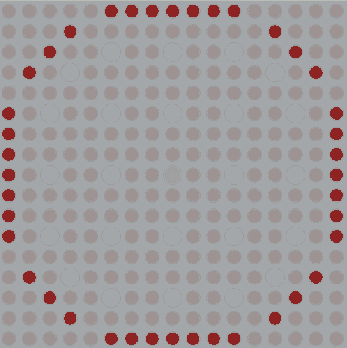
\includegraphics[width=0.9\linewidth]{figures/unsupervised/features/assm-16/u235-fiss/mean-spect-ind-sum/geometry-3}
  \caption{}
  \label{fig:chap10-fiss-mean-spect-ind-geom-3}
\end{subfigure}%
\begin{subfigure}{0.45\textwidth}
  \centering
  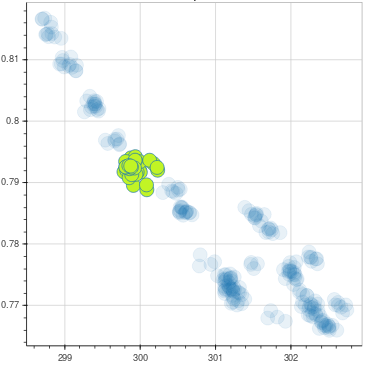
\includegraphics[width=0.9\linewidth]{figures/unsupervised/features/assm-16/u235-fiss/mean-spect-ind-sum/mgxs-3}
  \caption{}
  \label{fig:chap10-fiss-mean-spect-ind-mgxs-3}
\end{subfigure}
\caption[Clustering of U-235 fission MGXS spectral indices]{Scatter plots of the pin-wise U-235 fission (group 2 of 2) \ac{MGXS} means ($x$) and spectral indices ($y$) for the 1.6\% enriched fuel assembly.}
\label{fig:chap10-fiss-mean-spect-ind}
\end{figure}

%\clearpage

\begin{figure}[h!]
\centering
\begin{subfigure}{0.45\textwidth}
  \centering
  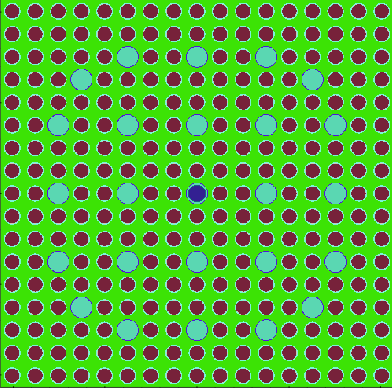
\includegraphics[width=0.9\linewidth]{figures/unsupervised/features/assm-16/geometry}
  \caption{}
  \label{fig:chap10-capt-mean-spect-ind-geom}
\end{subfigure}%
\begin{subfigure}{0.45\textwidth}
  \centering
  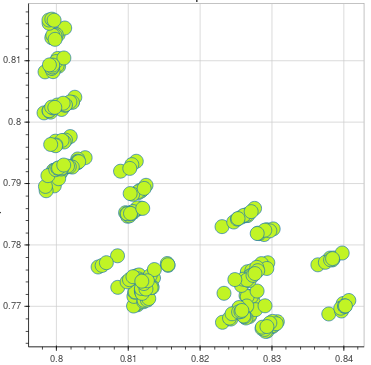
\includegraphics[width=0.9\linewidth]{figures/unsupervised/features/assm-16/u238-capt/mean-spect-ind-sum/mgxs}
  \caption{}
  \label{fig:chap10-capt-mean-spect-ind-mgxs}
\end{subfigure}
\begin{subfigure}{0.45\textwidth}
  \centering
  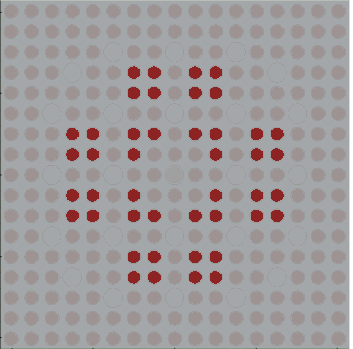
\includegraphics[width=0.9\linewidth]{figures/unsupervised/features/assm-16/u238-capt/mean-spect-ind-sum/geometry-2}
  \caption{}
  \label{fig:chap10-capt-mean-spect-ind-geom-2}
\end{subfigure}%
\begin{subfigure}{0.45\textwidth}
  \centering
  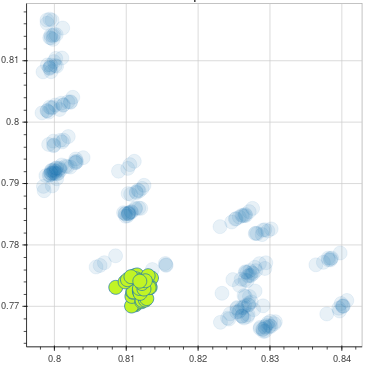
\includegraphics[width=0.9\linewidth]{figures/unsupervised/features/assm-16/u238-capt/mean-spect-ind-sum/mgxs-2}
  \caption{}
  \label{fig:chap10-capt-mean-spect-ind-mgxs-2}
\end{subfigure}
\begin{subfigure}{0.45\textwidth}
  \centering
  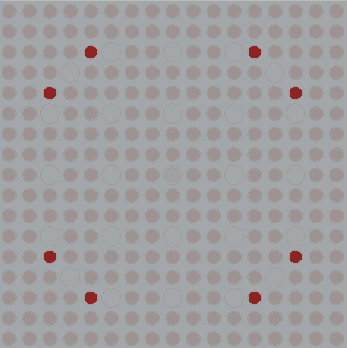
\includegraphics[width=0.9\linewidth]{figures/unsupervised/features/assm-16/u238-capt/mean-spect-ind-sum/geometry-3}
  \caption{}
  \label{fig:chap10-capt-mean-spect-ind-geom-3}
\end{subfigure}%
\begin{subfigure}{0.45\textwidth}
  \centering
  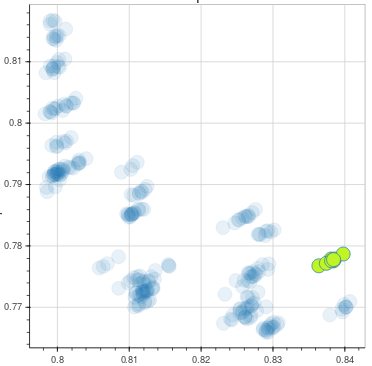
\includegraphics[width=0.9\linewidth]{figures/unsupervised/features/assm-16/u238-capt/mean-spect-ind-sum/mgxs-3}
  \caption{}
  \label{fig:chap10-capt-mean-spect-ind-mgxs-3}
\end{subfigure}
\caption[Clustering of U-238 capture MGXS spectral indices]{Scatter plots of the pin-wise U-238 capture (group 1 of 2) \ac{MGXS} means ($x$) and spectral indices ($y$) for the 1.6\% enriched fuel assembly.}
\label{fig:chap10-capt-mean-spect-ind}
\end{figure}

%\clearpage

The figures illustrate a complex relationship between the U-235 fission \ac{MGXS} and the spectral indices. In contrast to the fractional reactivity, both the fission and capture \ac{MGXS} are negatively correlated with the spectral index. In particular, the more differential moderation from neighboring \acp{CRGT}, the smaller the spectral index. Although the capture and fission rates both increase with differential moderation, these scatter plots indicate that U-235 fission increases \textit{faster} than U-238 capture. In addition, the clusters are more spread out than the more linear trends observed for the fractional reactivities. The scatter plots indicate that the spectral index is potentially more effective at separating sub-clusters within each primary cluster than fractional reactivity.

%(at least for this benchmark). 


%%%%%%%%%%%%%%%%%%%%%%%%%%%%%
\subsection{Nuclide Fraction}
\label{subsec:chap10-nuclide-frac}

The fractional reactivity and spectral index are both energy-integrated features, the \textit{nuclide fraction} feature is specific to each energy group. The nuclide fraction is defined as the ratio of each pin-wise microscopic \ac{MGXS} $\hat{\sigma}_{x,i,k,g}$ for reaction $x$, nuclide $i$ and energy group $k$ to the total \ac{MGXS} for the $\hat{\sigma}_{t,i,k,g}$ corresponding nuclide and energy group:

\begin{equation}
\label{eqn:chap10-nuclide-frac}
\hat{\tau}_{x,i,k,g} = \frac{\hat{\sigma}_{x,i,k,g}}{\hat{\sigma}_{t,i,k,g}}
\end{equation}

The nuclide fraction feature $\hat{\tau}_{x,i,k,g}$ is motivated by the hypothesis that spatial self-shielding effects may disproportionately impact certain reaction types (\textit{e.g.}, U-238 capture) more than the total \ac{MGXS}. Since the nuclide fraction is computed for each energy group, it may be more challenging to identify clusters with this feature with ``noisy'' \ac{MC} tally data than may be the case for the energy-integrated fractional reactivity and spectral index features. Like the spectral index, the nuclide fraction may identify pins with similar flux shapes but very different flux magnitudes since it is the ratio of two pin-wise reaction rates.

\begin{figure}[h!]
\centering
\begin{subfigure}{0.45\textwidth}
  \centering
  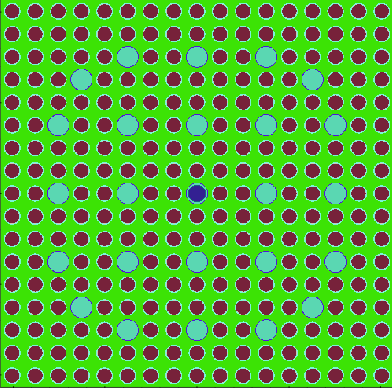
\includegraphics[width=0.9\linewidth]{figures/unsupervised/features/assm-16/geometry}
  \caption{}
  \label{fig:chap10-fiss-mean-nuc-frac-geom}
\end{subfigure}%
\begin{subfigure}{0.45\textwidth}
  \centering
  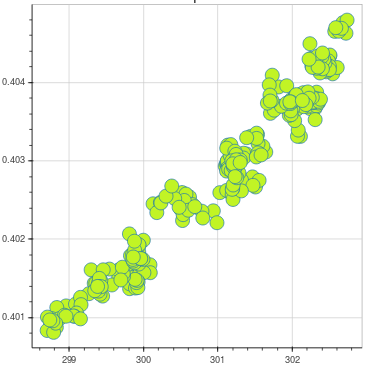
\includegraphics[width=0.9\linewidth]{figures/unsupervised/features/assm-16/u235-fiss/mean-nuc-frac/mgxs}
  \caption{}
  \label{fig:chap10-fiss-mean-nuc-frac-mgxs}
\end{subfigure}
\begin{subfigure}{0.45\textwidth}
  \centering
  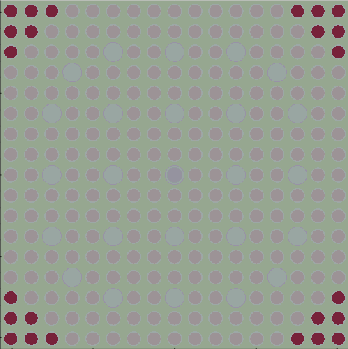
\includegraphics[width=0.9\linewidth]{figures/unsupervised/features/assm-16/u235-fiss/mean-nuc-frac/geometry-2}
  \caption{}
  \label{fig:chap10-fiss-mean-nuc-frac-geom-2}
\end{subfigure}%
\begin{subfigure}{0.45\textwidth}
  \centering
  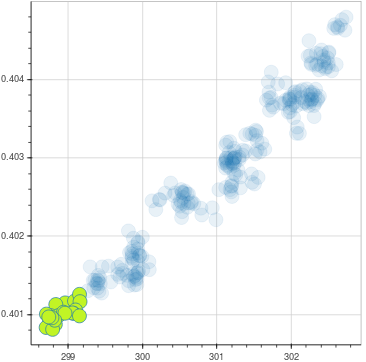
\includegraphics[width=0.9\linewidth]{figures/unsupervised/features/assm-16/u235-fiss/mean-nuc-frac/mgxs-2}
  \caption{}
  \label{fig:chap10-fiss-mean-nuc-frac-mgxs-2}
\end{subfigure}
\begin{subfigure}{0.45\textwidth}
  \centering
  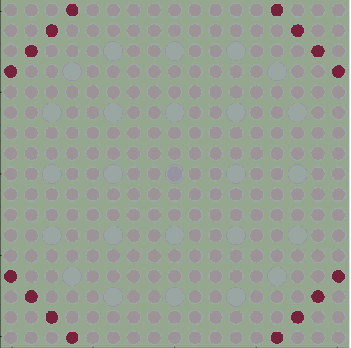
\includegraphics[width=0.9\linewidth]{figures/unsupervised/features/assm-16/u235-fiss/mean-nuc-frac/geometry-3}
  \caption{}
  \label{fig:chap10-fiss-mean-nuc-frac-geom-3}
\end{subfigure}%
\begin{subfigure}{0.45\textwidth}
  \centering
  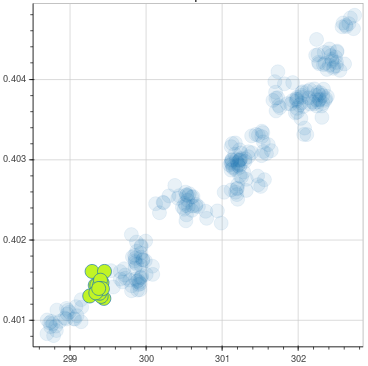
\includegraphics[width=0.9\linewidth]{figures/unsupervised/features/assm-16/u235-fiss/mean-nuc-frac/mgxs-3}
  \caption{}
  \label{fig:chap10-fiss-mean-nuc-frac-mgxs-3}
\end{subfigure}
\caption[Clustering of U-235 fission MGXS nuclide fractions]{Scatter plots of the pin-wise U-235 fission (group 2 of 2) \ac{MGXS} means ($x$) and nuclide fractions ($y$) for the 1.6\% enriched fuel assembly.}
\label{fig:chap10-fiss-mean-nuc-frac}
\end{figure}

%\clearpage

\begin{figure}[h!]
\centering
\begin{subfigure}{0.45\textwidth}
  \centering
  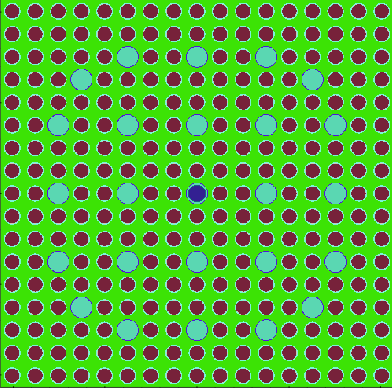
\includegraphics[width=0.9\linewidth]{figures/unsupervised/features/assm-16/geometry}
  \caption{}
  \label{fig:chap10-capt-mean-nuc-frac-geom}
\end{subfigure}%
\begin{subfigure}{0.45\textwidth}
  \centering
  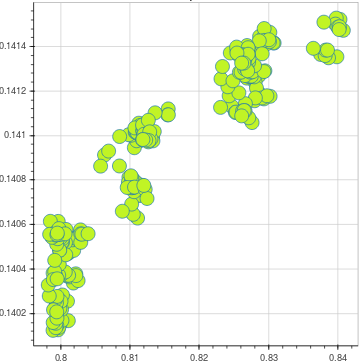
\includegraphics[width=0.9\linewidth]{figures/unsupervised/features/assm-16/u238-capt/mean-nuc-frac/mgxs}
  \caption{}
  \label{fig:chap10-capt-mean-nuc-frac-mgxs}
\end{subfigure}
\begin{subfigure}{0.45\textwidth}
  \centering
  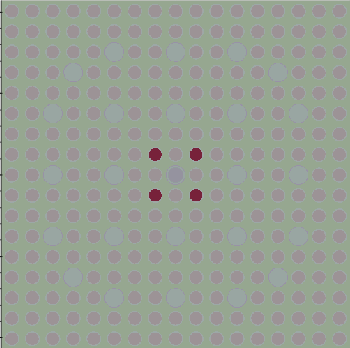
\includegraphics[width=0.9\linewidth]{figures/unsupervised/features/assm-16/u238-capt/mean-nuc-frac/geometry-2}
  \caption{}
  \label{fig:chap10-capt-mean-nuc-frac-geom-2}
\end{subfigure}%
\begin{subfigure}{0.45\textwidth}
  \centering
  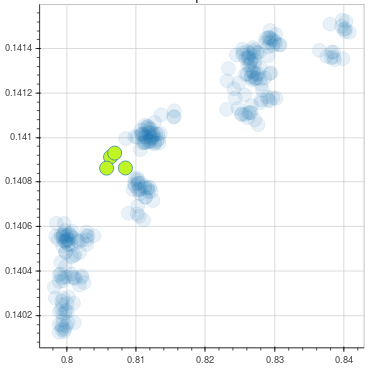
\includegraphics[width=0.9\linewidth]{figures/unsupervised/features/assm-16/u238-capt/mean-nuc-frac/mgxs-2}
  \caption{}
  \label{fig:chap10-capt-mean-nuc-frac-mgxs-2}
\end{subfigure}
\begin{subfigure}{0.45\textwidth}
  \centering
  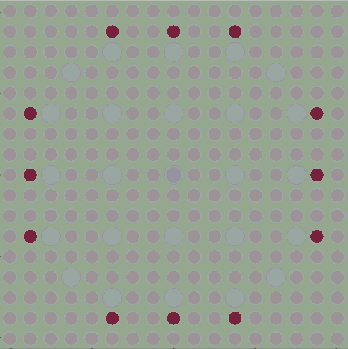
\includegraphics[width=0.9\linewidth]{figures/unsupervised/features/assm-16/u238-capt/mean-nuc-frac/geometry-3}
  \caption{}
  \label{fig:chap10-capt-mean-nuc-frac-geom-3}
\end{subfigure}%
\begin{subfigure}{0.45\textwidth}
  \centering
  \includegraphics[width=0.9\linewidth]{figures/unsupervised/features/assm-16/u238-capt/mean-nuc-frac/mgxs-3}
  \caption{}
  \label{fig:chap10-capt-mean-nuc-frac-mgxs-3}
\end{subfigure}
\caption[Clustering of U-238 capture MGXS nuclide fractions]{Scatter plots of the pin-wise U-238 capture (group 1 of 2) \ac{MGXS} means ($x$) and nuclide fractions ($y$) for the 1.6\% enriched fuel assembly.}
\label{fig:chap10-capt-mean-nuc-frac}
\end{figure}

%\clearpage

The nuclide fraction feature is illustrated with scatter plots in Figs.~\ref{fig:chap10-fiss-mean-nuc-frac} and~\ref{fig:chap10-capt-mean-nuc-frac} for 2-group U-235 fission and U-238 capture \ac{MGXS} data, respectively. The scatter plots include a single data point for each of the 264 fuel pins in the 1.6\% enriched fuel assembly benchmark. The $x$ and $y$ coordinates correspond to the tallied \ac{MGXS} means $\hat{\sigma}_{x,i,k,g}$ and nuclide fractions $\beta_{k}$, respectively. The complete datasets are illustrated in Figs.~\ref{fig:chap10-fiss-mean-nuc-frac-mgxs} and~\ref{fig:chap10-capt-mean-nuc-frac-mgxs}. The interactive \textit{i}\ac{MGXS} visualization tool was used to select clusters of \ac{MGXS} and plot the geometry to indicate the associated fuel pins, as displayed in Figs.~\Crefrange{fig:chap10-fiss-mean-nuc-frac-geom-2}{fig:chap10-fiss-mean-nuc-frac-mgxs-3} and~\Crefrange{fig:chap10-capt-mean-nuc-frac-geom-2}{fig:chap10-capt-mean-nuc-frac-mgxs-3} for the fission and capture \ac{MGXS}, respectively. 

The figures illustrate a positive correlation between both the U-235 fission and U-238 capture \ac{MGXS} and the nuclide fractions (at least for this benchmark). In particular, the more differential moderation from neighboring \acp{CRGT}, the smaller the larger the nuclide fraction. Although the fission, capture and total rates all increase with differential moderation, these scatter plots indicate that U-235 fission and U-238 capture increases \textit{faster} than the corresponding total reaction rates with U-235 and U-238. The clusters are more spread out than the more linear trends observed for the fractional reactivities, but this is likely due to the relatively larger statistical uncertainty for the energy-specific nuclide fractions than the energy-integrated fractional reactivities.

%%%%%%%%%%%%%%%%%%%%%%%%%%%%
%\subsection{Total Fraction}
%\label{subsec:chap10-tot-frac}
%
%first paragraph: explain what it is
%-divide pin-wise micro \ac{MGXS} for each nuclide/reaction/group by the corresponding total \ac{MGXS} for that nuclide/reaction/group trio
%-Eqn.~\ref{eqn:chap10-tot-frac}
%-explain what it indicates...???
%-note that $I$ designates the total number of nuclides in a fuel pin
%
%\begin{equation}
%\label{eqn:chap10-tot-frac}
%\omega_{x,i,k,g} = \frac{\hat{\sigma}_{x,i,k,g}}{\displaystyle\sum\limits_{i=1}^{I}\hat{\sigma}_{t,i,k,g}}
%\end{equation}

%%%%%%%%%%%%%%%%%%%%%%%%%%%%%%%%%%%%%%%%
\subsection{Feature Vector Construction}
\label{subsec:chap10-feature-eng-summary}

Each of the features described in the preceding sections is assembled into feature vectors for each sample as illustrated in Fig.~\ref{fig:chap10-features-example}. From a practical standpoint, the \textit{i}\ac{MGXS} implementation in this thesis represents the sample feature vectors with a 2D \texttt{DataFrame} object from the Pandas module~\cite{mckinney2010pandas} for data processing in Python. Each column in the \texttt{DataFrame} corresponds to a feature, and each row corresponds to a sample. This \texttt{DataFrame} is the input to the feature selection stage of the \textit{i}\ac{MGXS} pipeline. However, each feature must first be \textit{standardized} before used as an input to a predictive model.

\begin{figure}[h!]
\centering
\includegraphics[width=0.95\linewidth]{figures/unsupervised/features/engineering/features}
\vspace{2mm}
\caption[Example \textit{i}MGXS sample feature vectors]{\textit{i}\ac{MGXS} feature extraction computes fractional reactivities $\hat{\alpha}_{k}$, spectral indices $\hat{\beta}_{k}$, nuclide fractions $\hat{\tau}_{x,i,k,g}$, \ac{MGXS} means $\hat{\sigma}_{x,i,k,g}$ and standard deviations $\sigma_{\hat{\sigma}_{x,i,k,g}}$.}
\label{fig:chap10-features-example}
\end{figure}

Feature standardization -- also known as \textit{mean removal} and/or \textit{variance scaling} -- is commonly needed since many machine learning estimators assume that all features are centered about zero with near unit variance. In the context of \textit{i}\ac{MGXS}, the distance between samples (or clusters) in feature space will be skewed if the features are not standardized. In particular, the distance will be dominated by features with the largest magnitudes (\textit{e.g.}, thermal U-235 fission \ac{MGXS}), and conversely, insensitive to features with small magnitudes (\textit{e.g.}, \ac{MGXS} standard deviations). The canonical form of standardization \textit{translates} each sample by subtracting the mean $\overline{\hat{f}_{j}}$, and \textit{scales} each sample by dividing by the standard deviation $\sigma_{\hat{f}_{j}}$ of feature $j$:

\begin{equation}
\label{eqn:chap10-standard-standardize}
\hat{f}_{j,k}^{*} = \frac{\hat{f}_{j,k} - \overline{\hat{f}_{j}}}{\sigma_{\hat{f}_{j}}}
\end{equation}

\noindent where $\hat{f}_{j,k}^{*}$ is the standardized feature $j$ for fuel pin instance $k$. Several standardization schemes are provided by the \texttt{sklearn.preprocessing} module of the \texttt{scikit-learn} Python package for machine learning~\cite{pedregosa2011sklearn}. The \textit{i}\ac{MGXS} implementation in this thesis uses the \texttt{RobustScaler} to subtract the median and divide by the interquartile range (IQR)\footnote{The interquartile range is the difference between the first and third quartiles: $\mathrm{IQR} = Q_{3} - Q_{1}$.} to diminish the influence of outliers on the standardization process:

\begin{equation}
\label{eqn:chap10-robust-standardize}
\hat{f}_{j,k}^{*} = \frac{\hat{f}_{j,k} - \mathrm{median}\left\lbrace\hat{f}_{j,1}, \hat{f}_{j,2}, \dots, \hat{f}_{j,K}\right\rbrace}{\mathrm{IQR}_{\hat{f}_{j}}}
\end{equation}

\begin{emphbox}
\textbf{Features are random variables derived from \ac{MC} tally data which may provide information about \ac{MGXS} clustering. Feature vectors are constructed for each fuel pin instance and used as inputs for predictive clustering models.}
\end{emphbox}


%%%%%%%%%%%%%%%%%%%%%%%%%%%%%%%%%%%%%%%%%%%%%%%%%%%%%%%%%%%%%%%%%%%%%%%%%%%%%%%
\section{Feature Selection}
\label{sec:chap10-feature-select}

The \textit{feature selection} stage in the data processing pipeline in Fig.~\ref{fig:chap10-pipeline} determines which features to use when training\footnote{In machine learning, \textit{training} a model refers to the process of assigning numerical values to the parameters of the model to best fit an empirical dataset.} a clustering model. The feature extraction stage provides many different features, some of which may be poor predictors of \ac{MGXS} clusters. In addition, some features may be highly correlated and redundant as input variables to a predictive model. Feature selection attempts to identify the smallest possible subset of features necessary to achieve the desired predictive accuracy. Feature selection plays an important role in balancing the canonical \textit{bias--variance tradeoff} in statistics and machine learning by reducing model variance, while potentially increasing model bias. In particular, feature selection is used to train simple(r) machine learning models for the following three reasons:

\begin{itemize}[noitemsep]
\item \textbf{Reduce Model Complexity} -- Simpler models are easier to intuit and explain.
\item \textbf{Reduce Generalization Error} -- Simpler models reduce the risk of over-fitting.
\item \textbf{Reduce Training Time} -- Simpler models are computationally efficient to train.
\end{itemize}

Automated feature selection methods are often classified into three main categories: \textit{filter}, \textit{wrapper}, and \textit{embedded} methods. \textit{Filter methods} are agnostic to the family of predictive models one wishes to train and selects features which provide the most information about a target variable. Correlation Feature Selection~\cite{hall1999correlation} is an example of a filter method which searches for the smallest subset of features which are highly correlated with the target variable, but uncorrelated with each other. In contrast to filter methods, \textit{wrapper methods} evaluate subsets of features to determine their collective ability to minimize the generalization error of some specific family of predictive models. Wrapper methods may be computationally expensive since it entails a search of the space of possible feature subsets. In addition, wrapper methods may be at greater risk of over-fitting than filter methods since the feature selection criteria is based on model accuracy. Finally, \textit{embedded methods} select features as an integral part of the model training procedure. Some examples of embedded methods include $\ell_{1}$-regularization techniques and Recursive Feature Elimination~\cite{guyon2002rfe}. The interested reader is referred to~\cite{guyon2003select} or the plethora of other sources in the literature for more detailed information about automated feature selection methods.

This thesis makes a fairly limited use of feature selection techniques in its implementation of \textit{i}\ac{MGXS}. In particular, a number of relatively simple filter and wrapper methods are presented in the following sections as options to select the best features. This process is illustrated as part of the \textit{i}\ac{MGXS} data processing pipeline in Fig.~\ref{fig:chap10-select}. Sec.~\ref{subsec:chap10-litmus} presents \textit{litmus tests} to filter the features and choose those pairings of nuclides and reaction types which are most likely to exhibit clustering. Sec.~\ref{subsec:chap10-var-threshold} introduces variance thresholding, while Sec.~\ref{subsec:chap10-univariate-selection} highlights a collection of filter methods which select the highest scoring features. Sec.~\ref{subsec:chap10-select-from-model} discusses a wrapper method which selects features based on their importances for decision tree or ensemble regressors. Finally, while domain knowledge is not an automated approach to feature downselection, it is employed by the case studies in the following chapter and is discussed in Sec.~\ref{subsec:chap10-domain-knowledge}.

%Sec.~\ref{subsec:chap10-litmus-tot-frac} introduces a threshold-based method to downselect those nuclides with the most relevant data to cluster for a given energy group. Similarly, Sec.~\ref{subsec:chap10-litmus-nuc-frac} presents a threshold for the nuclide fraction to choose the ``best'' reaction type to cluster for a given nuclide and energy group.

\begin{figure}[h!]
\centering
\includegraphics[width=0.95\linewidth]{figures/unsupervised/features/engineering/select}
\vspace{2mm}
\caption[\textit{i}MGXS feature selection]{Feature selection chooses the features used to train a clustering model.}
\label{fig:chap10-select}
\end{figure}

It is important to note that the methods and metrics highlighted here should be considered an exhaustive list of options for feature selection for \textit{i}\ac{MGXS}. Furthermore, while all of the options discussed are supported in the \textit{i}\ac{MGXS} for this thesis, out of practical necessity only a few of the methods are evaluated by the empirical cases studies in this and the following chapter. Future work may aim to provide a more systematic appraisal of various feature selection methods for the \textit{i}\ac{MGXS} pipeline.

%%%%%%%%%%%%%%%%%%%%%%%%%%%%%%%%%%%%%%%%
\subsection{Litmus Tests}
\label{subsec:chap10-litmus}

\textit{Litmus tests} are filter methods specifically designed to select data for particular nuclides and reaction types for clustering. The litmus tests presented here are used to downselect the \ac{MGXS} mean and standard deviation features by predicting which nuclides and reaction types are most likely to exhibit clustering effects. The litmus tests are independently applied to each nuclide / energy group / reaction type trio. Sec.~\ref{subsubsec:chap10-litmus-tot-frac} introduces total fraction thresholding to select a nuclide for a given energy group, while Sec.~\ref{subsubsec:chap10-litmus-nuc-frac} introduces nuclide fraction thresholding to select a reaction type for a given nuclide and energy group. Sec.~\ref{subsubsec:chap10-litmus-nuc-frac} discusses how normality tests can be used to reject features which may have been drawn from a normal distribution.

%%%%%%%%%%%%%%%%%%%%%%%%%%%%%%%%%%%%%%%%
\subsubsection{Total Fraction Thresholding}
\label{subsubsec:chap10-litmus-tot-frac}

\textit{Total fraction thresholding} is a filter method used to select \ac{MGXS}-based features\footnote{\ac{MGXS}-based features include the microscopic \ac{MGXS} means $\hat{\sigma}_{x,i,k,g}$ and standard deviations $\sigma_{\hat{\sigma}_{x,i,k,g}}$, as well as the nuclide fraction $\hat{\tau}_{x,i,k,g}$.} for one or more nuclides for a particular energy group $g$ and reaction type $x$.
The total fraction gives an indication of how much a particular nuclide contributes to the total \ac{MGXS}. 
The \textit{total fraction} $\hat{\omega}_{x,i,k,g}$ is defined as the ratio of a macroscopic \ac{MGXS} $\hat{\Sigma}_{x,i,k,g}$ for nuclide $i$ and fuel pin instance $k$ to the total macroscopic \ac{MGXS} for all nuclides:

\begin{equation}
\label{eqn:chap10-tot-frac}
\hat{\omega}_{x,i,k,g} = \frac{\hat{\Sigma}_{x,i,k,g}}{\displaystyle\sum\limits_{i=1}^{I}\hat{\Sigma}_{t,i,k,g}}
\end{equation}

The \textit{i}\ac{MGXS} implementation in this thesis simply chooses \ac{MGXS}-based features for nuclide $i$ if the mean $\overline{\hat{\omega}}_{x,i,g}$ across fuel pins is greater than some user-defined threshold. This litmus test assumes that nuclide(s) which contribute little to the total \ac{MGXS} are likely not important to cluster. This assumption may not always be valid if some small \ac{MGXS} disproportionately reflect spatial self-shielding effects. For example, if the flux is appreciably depressed in narrow resonance groups for nuclides and reaction types which are especially sensitive to spatial self-shielding (\textit{e.g.}, U-238 capture), then the \ac{MGXS} may likewise be depressed such that the total fraction drops below the threshold and the feature(s) are neglected. The case studies explored in the following chapter use a relatively conservative value of 0.1 for the threshold such that \ac{MGXS}-based features for trace nuclides (\textit{e.g.}, O-17, U-234) are neglected and the \ac{MGXS} for U-235 and U-238 are always selected.

%This is unlikely, however, since spatial self-shielding effects are only manifested as clusters in pin-wise \ac{MGXS} if the continuous energy data varies over a relatively large range for a given energy group. A widely varying cross section, such as those in the resonance regime, will most likely result in a relatively large microscopic \ac{MGXS} and total fraction for the nuclide.

%%%%%%%%%%%%%%%%%%%%%%%%%%%%%%%%%%%%%%%%%%
\subsubsection{Nuclide Fraction Thresholding}
\label{subsubsec:chap10-litmus-nuc-frac}

first paragraph:
-filter method!!!
-used to choose reaction type: threshold on $\tau_{x,i,k,g}$
-motivate as automated selection of nuclide/reaction/energy group trios if *not* using pinch clustering
-only choose reactions which contribute at least some amount towards the total cross section
  -assumes that reaction(s) with little contribution are not important to cluster anyway
  -but may mistakenly make approx that MGXS with small magnitudes don't disproportionately reflect self-shielding effects
    -but this is a good assumption since larger MGXS will have smaller uncertainties anyway

%-threshold on the population variance divide by the population mean

%%%%%%%%%%%%%%%%%%%%%%%%%%%%
\subsubsection{Normality Tests}
\label{subsubsec:chap10-litmus-normality}

first paragraph: 
-used to choose 
-since all feature are tallied, makes assumption that population of feature realizations come from a normal distribution iff they do not reflect spatial self-shielding effects
-used to determine whether to cluster MGXS for a particular nuclide, group, rxn type
-look at $p$-value for Shapiro-Wilks tests of normality
-don't cluster data that may have come from a normal distribution!
-if the $p$-value is below a threshold, then data may be rejected as non-normal and may be good candidate for clustering

%%%%%%%%%%%%%%%%%%%%%%%%%%%%%%%%%%
\subsection{Variance Thresholding}
\label{subsec:chap10-var-threshold}

first paragraph:
-filter method!!!
-remove features with low variance
-\texttt{VarianceThreshold} class from \texttt{sklearn.feature_selection} module

%%%%%%%%%%%%%%%%%%%%%%%%%%%%%%%%%%
\subsection{Univariate Feature Selection}
\label{subsec:chap10-univariate-selection}

first paragraph:
-filter method!!!
-applies tests to features individually and selects those with highest scores
-does not consider correlations between features - e.g., could choose highly redundant features which each have high scores
-\texttt{GenericUnivariateSelect} class from \texttt{sklearn.feature_selection} module
-select $k$ best features, or highest percentage of features with highest scores
-also could use $\chi^2$ test or mutual information to select best features

%%%%%%%%%%%%%%%%%%%%%%%%%%%%%%%%%%
\subsection{Select From Model}
\label{subsec:chap10-select-from-model}

first paragraph:
-wrapper method!!!
-uses meta-transformer to select features based on importance weights
-\texttt{SelectFromModel} class from \texttt{sklearn.feature_selection} module
-train regression model to take any non-\ac{MGXS} mean features to map to \ac{MGXS} mean target variables
  -use \texttt{DecisionTreeRegressor} from \texttt{sklearn.tree}
    -choose features which correspond to nodes in tree which define biggest splits of dataset
  -use \texttt{RandomForestRegressor} from \texttt{sklearn.ensemble} to avoid over-fitting trees
    -choose features which correspond to nodes in tree which define biggest splits of dataset

%%%%%%%%%%%%%%%%%%%%%%%%%%%%%
\subsection{Domain Knowledge}
\label{subsec:chap10-domain-knowledge}

first paragraph: pinch clustering
-user selects a nuclide/reaction/energy/group trio(s)
  -instead, user will indicate wish to cluster individual MGXS like U-238 capture  
-use domain knowledge about which \ac{MGXS} are most sensitive to spatial self-shielding
  -MAY also reflect domain knowledge about which \ac{MGXS} are most important to cluster to best prediction reaction rates (e.g., U-238 capture)
  -and/or the \ac{MGXS} which are best *predictors* of the clustering of those \ac{MGXS} which are most important to cluster
-in this thesis just includes a single nuclide, reaction and energy group
  -e.g., U-238 capture in group 1/2
-could foreseeably mean multiple specific nuclides, reactions and energy groups

SUMMARY BOXES!!!


%%%%%%%%%%%%%%%%%%%%%%%%%%%%%%%%%%%%%%%%%%%%%%%%%%%%%%%%%%%%%%%%%%%%%%%%%%%%%%%
\section{Feature Agglomeration}
\label{sec:chap10-feature-agglomerate}

first paragraph: what is goal???
-curse of dimensionality - dimensionality reduction
-transform number of features to find new ones with more descriptive power than original set
  -new features may be more easily ordered than original ones
    -allowing for easier feature selection (Sec.~\ref{sec:chap10-litmus})
-can account for correlations between features
  -rather than treating each features independent

\begin{figure}[h!]
\centering
\includegraphics[width=0.95\linewidth]{figures/unsupervised/features/engineering/agglomerate}
\vspace{2mm}
\caption[\textit{i}MGXS feature agglomeration]{Agglomeration transforms the original feature vectors into new features.}
\label{fig:chap10-agglomerate}
\end{figure}

%%%%%%%%%%%%%%%%%%%%%%%%%%%%%%%%%%
\subsection{Feature Decomposition}
\label{subsec:chap10-feature-decomp}

%%%%%%%%%%%%%%%%%%%%%%%%%%%%%%%%%%%%%%%%%%%%
\subsubsection{Principal Component Analysis}
\label{subsubsec:chap10-feature-pca}

%%%%%%%%%%%%%%%%%%%%%%%%%%%%%%%%%%%%%%%%%%%%%%
\subsubsection{Independent Component Analysis}
\label{subsubsec:chap10-feature-transform-ica}

%%%%%%%%%%%%%%%%%%%%%%%%%%%%%%%%%%%%%%%
\subsection{Feature Importance Ranking}
\label{subsec:chap10-feature-importance}

%%%%%%%%%%%%%%%%%%%%%%%%%%%%%%%%%%%%%%%%
\subsubsection{Decision Tree Regression}
\label{subsubsec:chap10-decision-trees}

%%%%%%%%%%%%%%%%%%%%%%%%%%%%%%%%%%%
\subsubsection{Ensemble Regression}
\label{subsubsec:chap10-ensemble-methods}


%%%%%%%%%%%%%%%%%%%%%%%%%%%%%%%%%%%%%%%%%%%%%%%%%%%%%%%%%%%%%%%%%%%%%%%%%%%%%%%
\section{Clustering Feature Vectors}
\label{sec:chap10-clustering-algorithms}

-very brief overview
-refer to literature for more info
-used canned algorithms in scikit-learn \texttt{sklearn.cluster}
-while there are many, many algorithms out there, only a few selected for discussion here
  -one concern is scalability to large number of samples

\begin{figure}[h!]
\centering
\includegraphics[width=0.95\linewidth]{figures/unsupervised/features/engineering/cluster}
\vspace{2mm}
\caption[\textit{i}MGXS clustering]{Each clustering model assigns labels to each sample.}
\label{fig:chap10-cluster}
\end{figure}

%%%%%%%%%%%%%%%%%%%%%%%%%%%%%%%%%%%%%%%%%%%%%%%%%%%%%%%%%%%%%%%%%%%%%%%%%%%%%%%
\subsection{Unsupervised Clustering}
\label{subsec:chap10-feature-mapping}

%%%%%%%%%%%%%%%%%%%%%%%%%%%%%%%%%
\subsubsection{$k$-Means Clustering}
\label{subsubsec:chap10-kmeans}

-introduce scheme
-algorithmic
-initialization
-model selection

%%%%%%%%%%%%%%%%%%%%%%%%%%%%%%%%%%%%
\subsubsection{Hierarchical Clustering}
\label{subsubsec:chap10-agglomerative}

-introduce scheme
-algorithmic
-initialization
-model selection

%%%%%%%%%%%%%%%%%%%%%%%%%%%%
\subsubsection{DBSCAN}
\label{subsubsec:chap10-dbscan}

-introduce scheme
-algorithmic
-initialization
-model selection

%%%%%%%%%%%%%%%%%%%%%%%%%%%%
\subsubsection{Birch}
\label{subsubsec:chap10-birch}

-introduce scheme
-algorithmic
-initialization
-model selection

%%%%%%%%%%%%%%%%%%%%%%%%%%%%%%%%%
\subsubsection{Gaussian Mixture Models}
\label{subsubsec:chap10-gmms}

-introduce scheme
-algorithmic
-initialization
-intro fact that it is not scalable - not evaluated here
-mention dirichlet process mixture models
-model selection criteria are nice
-model selection

%%%%%%%%%%%%%%%%%%%%%%%%%%%%%%%%%%%%%%%%%%%%%%%%%%%%%%%%%%%%%%%%%%%%%%%%%%%%%%%
\subsubsection{Mapping Features to MGXS Targets}
\label{subsubsec:chap10-feature-mapping}

%-competing paradigms:
%  -clustering
%  -input -> target (e.g., trees)
%  -some combination of the two


%%%%%%%%%%%%%%%%%%%%%%%%%%%%%%%%%%%%%%%%%%%%%%%%%%%%%%%%%%%%%%%%%%%%%%%%%%%%%%%
\section{Model Selection}
\label{sec:chap10-model-select}

\begin{figure}[h!]
\centering
\includegraphics[width=0.95\linewidth]{figures/unsupervised/features/engineering/model}
\vspace{2mm}
\caption[\textit{i}MGXS model selection]{Model selection evaluates the clustering models.}
\label{fig:chap10-model}
\end{figure}


%%%%%%%%%%%%%%%%%%%%%%%%%%%%%%%%%%%%%%%%%%%%%%%%%%%%%%%%%%%%%%%%%%%%%%%%%%%%%%%
\section{\textit{i}\ac{MGXS} Spatial Homogenization}
\label{sec:chap10-imgxs-pipeline}

\begin{figure}[h!]
\centering
\includegraphics[width=0.95\linewidth]{figures/unsupervised/features/engineering/flow-chart}
\vspace{2mm}
\caption[\textit{i}MGXS flow chart]{The complete \textit{i}\ac{MGXS} flow chart.}
\label{fig:chap10-flow-chart}
\end{figure}


%%%%%%%%%%%%%%%%%%%%%%%%%%%%%%%%%%%%%%%%%%%%%%%%%%%%%%%%%%%%%%%%%%%%%%%%%%%%%%%
\section{Clustered Geometries}
\label{sec:chap10-geometries}

-agglomerative clustering was used to generate the figures
-which nuclide, group, reaction was used for pinch clustering???

\begin{figure}[h!]
\centering
\begin{subfigure}{0.48\textwidth}
  \centering
  \includegraphics[width=0.9\linewidth]{figures/unsupervised/geometries/with-features/2-clusters/pinch/assm-16}
  \caption{}
  \label{fig:chap10-assm-16-pinch-2}
\end{subfigure}%
\begin{subfigure}{0.48\textwidth}
  \centering
  \includegraphics[width=0.9\linewidth]{figures/unsupervised/geometries/with-features/2-clusters/combined/assm-16}
  \caption{}
  \label{fig:chap10-assm-16-combined-2}
\end{subfigure}
\begin{subfigure}{0.48\textwidth}
  \centering
  \includegraphics[width=0.9\linewidth]{figures/unsupervised/geometries/with-features/4-clusters/pinch/assm-16}
  \caption{}
  \label{fig:chap10-assm-16-pinch-4}
\end{subfigure}%
\begin{subfigure}{0.48\textwidth}
  \centering
  \includegraphics[width=0.9\linewidth]{figures/unsupervised/geometries/with-features/4-clusters/combined/assm-16}
  \caption{}
  \label{fig:chap10-assm-16-combined-4}
\end{subfigure}
\begin{subfigure}{0.48\textwidth}
  \centering
  \includegraphics[width=0.9\linewidth]{figures/unsupervised/geometries/with-features/8-clusters/pinch/assm-16}
  \caption{}
  \label{fig:chap10-assm-16-pinch-8}
\end{subfigure}%
\begin{subfigure}{0.48\textwidth}
  \centering
  \includegraphics[width=0.9\linewidth]{figures/unsupervised/geometries/with-features/8-clusters/combined/assm-16}
  \caption{}
  \label{fig:chap10-assm-16-combined-8}
\end{subfigure}
\caption[Materials for the 1.6\% fuel assembly with clustering homogenization]{Materials for the 1.6\% enriched fuel assembly with clustering homogenization. The materials for 2, 4, and 8 clusters are illustrated in (a), (c) and (e) for pinch clustering, and in (b), (d) and (f) for combined clustering, respectively.}
\label{fig:chap10-assm-16-geometries}
\end{figure}

\clearpage

\begin{figure}[h!]
\centering
\begin{subfigure}{0.48\textwidth}
  \centering
  \includegraphics[width=0.9\linewidth]{figures/unsupervised/geometries/with-features/2-clusters/pinch/assm-31-20BPs}
  \caption{}
  \label{fig:chap10-assm-31-20BPs-pinch-2}
\end{subfigure}%
\begin{subfigure}{0.48\textwidth}
  \centering
  \includegraphics[width=0.9\linewidth]{figures/unsupervised/geometries/with-features/2-clusters/combined/assm-31-20BPs}
  \caption{}
  \label{fig:chap10-assm-31-20BPs-combined-2}
\end{subfigure}
\begin{subfigure}{0.48\textwidth}
  \centering
  \includegraphics[width=0.9\linewidth]{figures/unsupervised/geometries/with-features/4-clusters/pinch/assm-31-20BPs}
  \caption{}
  \label{fig:chap10-assm-31-20BPs-pinch-4}
\end{subfigure}%
\begin{subfigure}{0.48\textwidth}
  \centering
  \includegraphics[width=0.9\linewidth]{figures/unsupervised/geometries/with-features/4-clusters/combined/assm-31-20BPs}
  \caption{}
  \label{fig:chap10-assm-31-20BPs-combined-4}
\end{subfigure}
\begin{subfigure}{0.48\textwidth}
  \centering
  \includegraphics[width=0.9\linewidth]{figures/unsupervised/geometries/with-features/8-clusters/pinch/assm-31-20BPs}
  \caption{}
  \label{fig:chap10-assm-31-20BPs-pinch-8}
\end{subfigure}%
\begin{subfigure}{0.48\textwidth}
  \centering
  \includegraphics[width=0.9\linewidth]{figures/unsupervised/geometries/with-features/8-clusters/combined/assm-31-20BPs}
  \caption{}
  \label{fig:chap10-assm-31-20BPs-combined-8}
\end{subfigure}
\caption[Materials for the 3.1\% fuel assembly with clustering homogenization]{Materials for the 3.1\% enriched fuel assembly with 20 \acp{BP} with clustering homogenization. The materials for 2, 4, and 8 clusters are illustrated in (a), (c) and (e) for pinch clustering, and in (b), (d) and (f) for combined clustering, respectively.}
\label{fig:chap10-assm-31-20BPs-geometries}
\end{figure}

\clearpage

\begin{figure}[h!]
\centering
\begin{subfigure}{0.48\textwidth}
  \centering
  \includegraphics[width=0.9\linewidth]{figures/unsupervised/geometries/with-features/2-clusters/pinch/2x2}
  \caption{}
  \label{fig:chap10-2x2-pinch-2}
\end{subfigure}%
\begin{subfigure}{0.48\textwidth}
  \centering
  \includegraphics[width=0.9\linewidth]{figures/unsupervised/geometries/with-features/2-clusters/combined/2x2}
  \caption{}
  \label{fig:chap10-2x2-combined-2}
\end{subfigure}
\begin{subfigure}{0.48\textwidth}
  \centering
  \includegraphics[width=0.9\linewidth]{figures/unsupervised/geometries/with-features/4-clusters/pinch/2x2}
  \caption{}
  \label{fig:chap10-2x2-pinch-4}
\end{subfigure}%
\begin{subfigure}{0.48\textwidth}
  \centering
  \includegraphics[width=0.9\linewidth]{figures/unsupervised/geometries/with-features/4-clusters/combined/2x2}
  \caption{}
  \label{fig:chap10-assm-2x2-combined-4}
\end{subfigure}
\begin{subfigure}{0.48\textwidth}
  \centering
  \includegraphics[width=0.9\linewidth]{figures/unsupervised/geometries/with-features/8-clusters/pinch/2x2}
  \caption{}
  \label{fig:chap10-assm-2x2-pinch-8}
\end{subfigure}%
\begin{subfigure}{0.48\textwidth}
  \centering
  \includegraphics[width=0.9\linewidth]{figures/unsupervised/geometries/with-features/8-clusters/combined/2x2}
  \caption{}
  \label{fig:chap10-assm-2x2-combined-8}
\end{subfigure}
\caption[Materials for the 2$\times$2 periodic colorset with clustering homogenization]{Materials for the 2$\times$2 periodic colorset with clustering homogenization. The materials for 2, 4, and 8 clusters are illustrated in (a), (c) and (e) for pinch clustering, and in (b), (d) and (f) for combined clustering, respectively.}
\label{fig:chap10-2x2-geometries}
\end{figure}

\clearpage

\begin{figure}[h!]
\centering
\begin{subfigure}{0.48\textwidth}
  \centering
  \includegraphics[width=0.9\linewidth]{figures/unsupervised/geometries/with-features/2-clusters/pinch/reflector}
  \caption{}
  \label{fig:chap10-reflector-pinch-2}
\end{subfigure}%
\begin{subfigure}{0.48\textwidth}
  \centering
  \includegraphics[width=0.9\linewidth]{figures/unsupervised/geometries/with-features/2-clusters/combined/reflector}
  \caption{}
  \label{fig:chap10-reflector-combined-2}
\end{subfigure}
\begin{subfigure}{0.48\textwidth}
  \centering
  \includegraphics[width=0.9\linewidth]{figures/unsupervised/geometries/with-features/4-clusters/pinch/reflector}
  \caption{}
  \label{fig:chap10-reflector-pinch-4}
\end{subfigure}%
\begin{subfigure}{0.48\textwidth}
  \centering
  \includegraphics[width=0.9\linewidth]{figures/unsupervised/geometries/with-features/4-clusters/combined/reflector}
  \caption{}
  \label{fig:chap10-reflector-combined-4}
\end{subfigure}
\begin{subfigure}{0.48\textwidth}
  \centering
  \includegraphics[width=0.9\linewidth]{figures/unsupervised/geometries/with-features/8-clusters/pinch/reflector}
  \caption{}
  \label{fig:chap10-reflector-pinch-8}
\end{subfigure}%
\begin{subfigure}{0.48\textwidth}
  \centering
  \includegraphics[width=0.9\linewidth]{figures/unsupervised/geometries/with-features/8-clusters/combined/reflector}
  \caption{}
  \label{fig:chap10-reflector-combined-8}
\end{subfigure}
\caption[Materials for the 2$\times$2 colorset with reflector with clustering homogenization]{Materials for the 2$\times$ colorset with water reflector with clustering homogenization. The materials for 2, 4, and 8 clusters are illustrated in (a), (c) and (e) for pinch clustering, and in (b), (d) and (f) for combined clustering, respectively.}
\label{fig:chap10-reflector-geometries}
\end{figure}

\clearpage

\begin{figure}[h!]
\centering
\begin{subfigure}{0.68\textwidth}
  \centering
  \includegraphics[width=\linewidth]{figures/unsupervised/geometries/with-features/2-clusters/pinch/full-core}
  \caption{}
  \label{fig:chap10-full-core-pinch-2}
\end{subfigure}
\begin{subfigure}{0.68\textwidth}
  \centering
  \includegraphics[width=\linewidth]{figures/unsupervised/geometries/with-features/2-clusters/combined/full-core}
  \caption{}
  \label{fig:chap10-full-core-combined-2}
\end{subfigure}
\caption[Materials for BEAVRS with clustering homogenization (2 clusters)]{Materials for the \ac{BEAVRS} model with \textit{i}\ac{MGXS} spatial homogenization from 2 clusters with pinch feature selection (a) and automated feature selection (b).}
\label{fig:chap10-full-core-geometries-2}
\end{figure}

\clearpage

\begin{figure}[h!]
\centering
\begin{subfigure}{0.68\textwidth}
  \centering
  \includegraphics[width=\linewidth]{figures/unsupervised/geometries/with-features/4-clusters/pinch/full-core}
  \caption{}
  \label{fig:chap10-full-core-pinch-4}
\end{subfigure}
\begin{subfigure}{0.68\textwidth}
  \centering
  \includegraphics[width=\linewidth]{figures/unsupervised/geometries/with-features/4-clusters/combined/full-core}
  \caption{}
  \label{fig:chap10-full-core-combined-4}
\end{subfigure}
\caption[Materials for BEAVRS with clustering homogenization (4 clusters)]{Materials for the \ac{BEAVRS} model with \textit{i}\ac{MGXS} spatial homogenization from 4 clusters with pinch feature selection (a) and automated feature selection (b).}
\label{fig:chap10-full-core-geometries-4}
\end{figure}

\clearpage

\begin{figure}[h!]
\centering
\begin{subfigure}{0.68\textwidth}
  \centering
  \includegraphics[width=\linewidth]{figures/unsupervised/geometries/with-features/8-clusters/pinch/full-core}
  \caption{}
  \label{fig:chap10-full-core-pinch-8}
\end{subfigure}
\begin{subfigure}{0.68\textwidth}
  \centering
  \includegraphics[width=\linewidth]{figures/unsupervised/geometries/with-features/8-clusters/combined/full-core}
  \caption{}
  \label{fig:chap10-full-core-combined-8}
\end{subfigure}
\caption[Materials for BEAVRS with clustering homogenization (8 clusters)]{Materials for the \ac{BEAVRS} model with \textit{i}\ac{MGXS} spatial homogenization from 8 clusters with pinch feature selection (a) and automated feature selection (b).}
\label{fig:chap10-full-core-geometries-8}
\end{figure}

\clearpage

\begin{figure}[h!]
\centering
\begin{subfigure}{0.68\textwidth}
  \centering
  \includegraphics[width=\linewidth]{figures/unsupervised/geometries/with-features/16-clusters/pinch/full-core}
  \caption{}
  \label{fig:chap10-full-core-pinch-16}
\end{subfigure}
\begin{subfigure}{0.68\textwidth}
  \centering
  \includegraphics[width=\linewidth]{figures/unsupervised/geometries/with-features/16-clusters/combined/full-core}
  \caption{}
  \label{fig:chap10-full-core-combined-16}
\end{subfigure}
\caption[Materials for BEAVRS with clustering homogenization (16 clusters)]{Materials for the \ac{BEAVRS} model with \textit{i}\ac{MGXS} spatial homogenization from 16 clusters with pinch feature selection (a) and automated feature selection (b).}
\label{fig:chap10-full-core-geometries-16}
\end{figure}

\clearpage

\begin{figure}[h!]
\centering
\begin{subfigure}{0.68\textwidth}
  \centering
  \includegraphics[width=\linewidth]{figures/unsupervised/geometries/with-features/32-clusters/pinch/full-core}
  \caption{}
  \label{fig:chap10-full-core-pinch-32}
\end{subfigure}
\begin{subfigure}{0.68\textwidth}
  \centering
  \includegraphics[width=\linewidth]{figures/unsupervised/geometries/with-features/32-clusters/combined/full-core}
  \caption{}
  \label{fig:chap10-full-core-combined-32}
\end{subfigure}
\caption[Materials for BEAVRS with clustering homogenization (32 clusters)]{Materials for the \ac{BEAVRS} model with \textit{i}\ac{MGXS} spatial homogenization from 32 clusters with pinch feature selection (a) and automated feature selection (b).}
\label{fig:chap10-full-core-geometries-32}
\end{figure}

\clearpage

\begin{figure}[h!]
\centering
\begin{subfigure}{0.68\textwidth}
  \centering
  \includegraphics[width=\linewidth]{figures/unsupervised/geometries/with-features/64-clusters/pinch/full-core}
  \caption{}
  \label{fig:chap10-full-core-pinch-64}
\end{subfigure}
\begin{subfigure}{0.68\textwidth}
  \centering
  \includegraphics[width=\linewidth]{figures/unsupervised/geometries/with-features/64-clusters/combined/full-core}
  \caption{}
  \label{fig:chap10-full-core-combined-64}
\end{subfigure}
\caption[Materials for BEAVRS with clustering homogenization (64 clusters)]{Materials for the \ac{BEAVRS} model with \textit{i}\ac{MGXS} spatial homogenization from 64 clusters with pinch feature selection (a) and automated feature selection (b).}
\label{fig:chap10-full-core-geometries-64}
\end{figure}

\clearpage

%%%%%%%%%%%%%%%%%%%%%%%%%%%%%%%%%%%%%%%%%%%%%%%%%%%%%%%%%%%%%%%%%%%%%%%%%%%%%%%
\section{Evaluating the Methodology}
\label{sec:chap10-cluster}

%%%%%%%%%%%%%%%%%%%%%%%%%%%%%%%
\subsection{Perfect Clustering}
\label{subsec:chap10-perfect-cluster}

%%%%%%%%%%%%%%%%%%%%%%%%%%%%%%%%
\subsection{Adaptive Clustering}
\label{subsec:chap10-adaptive-cluster}

\begin{itemize}[noitemsep]
  \item dataset restrictions
  \begin{itemize}[noitemsep]
    \item \textbf{``pinch'' clustering} - a \textit{single} nuclide/group/reaction triplet
    \item \textbf{``combined'' clustering} - one or more nuclide/group pairs \textit{together}
    \item \textbf{``local'' clustering} - one or more nuclide/group pairs \textit{separately}
  \end{itemize}
  \item clustering algorithms
  \begin{itemize}[noitemsep]
    \item discriminative clustering ($k$-Means++, Agglomerative, etc.)
    \item generative clustering (Gaussian Mixtures, Dirichlet Processes)
  \end{itemize}
  \item ``regression-informed'' clustering
  \begin{itemize}[noitemsep]
    \item use a regressor to predict ``smoothed'' of target variable(s)
    \begin{itemize}[noitemsep]
      \item decision tree regression
      \item ensemble (boosting, random forest) regression
      \item Gaussian Process regression
    \end{itemize}
    \item cluster predictions produced by regressor
    \item advantage is that objective function \textit{may} be more appropriate
  \end{itemize}
\end{itemize}